\documentclass{article}
\usepackage[margin=1in]{geometry}
\usepackage{amssymb}
\usepackage{etoolbox}
\usepackage{graphicx}
\usepackage{subfig}
\usepackage{algorithm}
\usepackage{algpseudocode}
\usepackage{float}
\usepackage{etoolbox}
\usepackage{tikz}
\usepackage{dsfont}
\usepackage{listings}
\definecolor{codegreen}{rgb}{0,0.6,0}
\definecolor{codegray}{rgb}{0.5,0.5,0.5}
\definecolor{codepurple}{rgb}{0.58,0,0.82}
\definecolor{backcolour}{rgb}{0.95,0.95,0.95}
\lstdefinestyle{code}{
	backgroundcolor=\color{backcolour},   
	commentstyle=\color{codegreen},
	keywordstyle=\color{magenta},
	numberstyle=\tiny\color{codegray},
	stringstyle=\color{codepurple},
	basicstyle=\ttfamily\footnotesize,
	breakatwhitespace=false,         
	breaklines=true,                 
	captionpos=b,              
	numbers=left,                    
	numbersep=5pt,
	frame=single,
}
\usetikzlibrary{tikzmark}
\usetikzlibrary{calc}

\errorcontextlines\maxdimen

% begin vertical rule patch for algorithmicx (http://tex.stackexchange.com/questions/144840/vertical-loop-block-lines-in-algorithmicx-with-noend-option)
% note that some of the packages above are also needed
\newcommand{\ALGtikzmarkcolor}{black}% customise this, if you want
\newcommand{\ALGtikzmarkextraindent}{4pt}% customise this, if you want
\newcommand{\ALGtikzmarkverticaloffsetstart}{-.5ex}% customise this, if you want
\newcommand{\ALGtikzmarkverticaloffsetend}{-.5ex}% customise this, if you want
\makeatletter
\newcounter{ALG@tikzmark@tempcnta}

\newcommand\ALG@tikzmark@start{%
	\global\let\ALG@tikzmark@last\ALG@tikzmark@starttext%
	\expandafter\edef\csname ALG@tikzmark@\theALG@nested\endcsname{\theALG@tikzmark@tempcnta}%
	\tikzmark{ALG@tikzmark@start@\csname ALG@tikzmark@\theALG@nested\endcsname}%
	\addtocounter{ALG@tikzmark@tempcnta}{1}%
}

\def\ALG@tikzmark@starttext{start}
\newcommand\ALG@tikzmark@end{%
	\ifx\ALG@tikzmark@last\ALG@tikzmark@starttext
	% ignore this, the block was opened then closed directly without any other blocks in between (so just a \State basically)
	% don't draw a vertical line here
	\else
	\tikzmark{ALG@tikzmark@end@\csname ALG@tikzmark@\theALG@nested\endcsname}%
	\tikz[overlay,remember picture] \draw[\ALGtikzmarkcolor] let \p{S}=($(pic cs:ALG@tikzmark@start@\csname ALG@tikzmark@\theALG@nested\endcsname)+(\ALGtikzmarkextraindent,\ALGtikzmarkverticaloffsetstart)$), \p{E}=($(pic cs:ALG@tikzmark@end@\csname ALG@tikzmark@\theALG@nested\endcsname)+(\ALGtikzmarkextraindent,\ALGtikzmarkverticaloffsetend)$) in (\x{S},\y{S})--(\x{S},\y{E});%
	\fi
	\gdef\ALG@tikzmark@last{end}%
}



% the following line injects our new tikzmarking code
\apptocmd{\ALG@beginblock}{\ALG@tikzmark@start}{}{\errmessage{failed to patch}}
\pretocmd{\ALG@endblock}{\ALG@tikzmark@end}{}{\errmessage{failed to patch}}
\makeatother
% end vertical rule patch for algorithmicx

\patchcmd{\thebibliography}{\section*{\refname}}{}{}{}
\usepackage{url}
\renewenvironment{abstract}
{\small
	\begin{center}
		\bfseries \abstractname\vspace{-.4em}
	\end{center}
	\list{}{
		\setlength{\leftmargin}{2cm}
		\setlength{\rightmargin}{\leftmargin}
	}
	\item\relax}
{\endlist}
\date{}
\begin{document}
	\begin{center}
		\large{\rule{420pt}{0.4pt}}\\
		\vspace{0.15in}
		\LARGE{\bfseries{Attention-Over-Actions Option-Critic}}
		\vspace{0.1in}
		\large{\rule{420pt}{0.4pt}}
		
		\large{IB Computer Science Extended Essay}
		
		\normalsize{Word Count:}
	\end{center}
	\vspace{0.1in}
	\section*{Research Question}
	How are localized options trained in the Option-Critic architecture? \\
	\vspace{0.1in}
	\section{Introduction}
	\qquad \ As human we operate in high level actions. For example when driving a car, we make decisions about turning left or right instead of thinking about which muscle to contract. Human have the ability to group a chain of actions into one single high level action. 
	
	\quad In Reinforcement Learning, we have a way to capture this idea of grouping action by using options \cite{SUTTON1999181}. When the options are defined, learning how to use them are very simple. However, if the options are not given and need to be learned, things get a lot harder since it requires knowing what makes an option good. 

	\quad Many people argue that a good options should be diverse and localized, and many recent algorithms have followed this argument. Indeed, these algorithms have been able to discover options that are localized, so in this essay, I will try to derive a framework for localization in order to answer my research question, and I will develop an algorithm out of the framework to see whether it can actually train localized options. 
	
	\quad This essay will be structured as follows: First, preliminary and related work will be presented to give a context to what I am trying to do. Second, previous work will be analyzed to figure out how localization is achieved. Third, a framework will be proposed based on the observations made in the analysis. Forth, an algorithm will be derived from the framework. Finally, the algorithm will be tested in the Four Rooms environment.
	\section{Preliminary}
	\qquad \ This section only acts as a summary. You are assumed to have basic knowledge about Reinforcement Learning and Options.
	\subsection*{Markov Decision Process}
	\qquad \ Markov decision process (MDP) \cite{sutton2018reinforcement} is a mathematical framework for modeling decision making in a stochastic environment. It is defined as a tuple: $<\mathcal{S}, \mathcal{A}, r, \gamma, P>$ where:
	
	$\mathcal{S}$ is the set of states.
	
	$\mathcal{A}$ is the set of actions
	
	$r : \mathcal{S} \times \mathcal{A} \rightarrow \mathbb{R}$ is the reward function
	
	$\gamma \in [0,1)$ is the discount factor that ensure the cumulative reward $\sum_{t=0}^{\infty} \gamma^t r(s_t, a_t)$ converges
	
	$P : \mathcal{S} \times A \times \mathcal{S} \rightarrow [0,1]$ is the transition model which gives the probability for a particular transition to occur.
	
	\quad All MDPs must follow the Markov Property, which means that everything is stateless and does not depend on the history. In an MDP, A policy $\pi : \mathcal{S} \times \mathcal{A} \rightarrow [0,1]$ is responsible for choosing the action, after an action is chosen, the environment transitions to a new state according to $P(s,a,s')$, and a reward is given to the policy. This process repeats until the environment enters a terminal state.
	\subsection*{Reinforcement Learning}
	\qquad \ Reinforcement Learning (RL) \cite{sutton2018reinforcement} is a machine learning paradigm which allows an agent to learn from interaction in an MDP. The agent's goal is to maximizes a certain objective function.
	
	\quad Actor-Critic \cite{Konda00actor-criticalgorithms} is one of the popular classes of algorithms that harvest the advantage of both Q-Learning and Policy Gradient. An actor network is trained to choose the best action, while a critic network is trained to evaluate the decision made by the actor network.
	\subsection*{Option Framework}
	\qquad \ In the Option Framework\cite{SUTTON1999181}, instead of only using 1 policy, we use a set of options, each option is defined as a tuple: $<\mathcal{I}_\omega,\pi_\omega,\beta_\omega>$, where:
	
	\qquad $\mathcal{I}_\omega \subseteq \mathcal{S}$ is the initiation set that define which state the option can be selected
	
	\qquad $\pi_\omega : \mathcal{S} \times \mathcal{A} \rightarrow [0,1]$ is the internal policy
	
	\qquad $\beta_\omega:\mathcal{S} \rightarrow [0,1]$ is the termination probability.
	
	\quad These options take turns to choose the action. A policy-over-options $\pi_\Omega : \mathcal{S} \times \Omega \rightarrow [0,1]$, where $\Omega$ is the set of options, decides which option to use. When an option is chosen, actions are chosen by its internal policy $\pi_\omega$ from then on, until it terminated according to its $\beta_\omega$, then the policy-over-options $\pi_\Omega$ chooses an option again. An option has a chance to terminate every time environment transitions to a new state.
	
	\quad If the options are defined, the policy-over-options $\pi_\Omega$ can be learned by using SMDP Q-Learning \cite{smdp} or Intra-Option Learning \cite{intraoplearn}. However, options are not always predefined and need to be discovered.
	\subsection*{Four Rooms Environment}
	\qquad \ The Four Rooms environment is commonly used to evaluate algorithms that use options. The agent have 4 actions: up, down, left and right, which will move the agent in that corresponding direction. The choice of agent has $1/3$ chance to fail and a random action will be chosen instead.
	
	\quad +50 reward will be given to the agent when it arrives to the goal state, and the episode will terminate after that.
	
	\quad Each cell position in the environment is mapped to a state number and is given to the agent in each step. The agent starts in a random state when an episode starts.
	\begin{figure}[h]
		\centering
		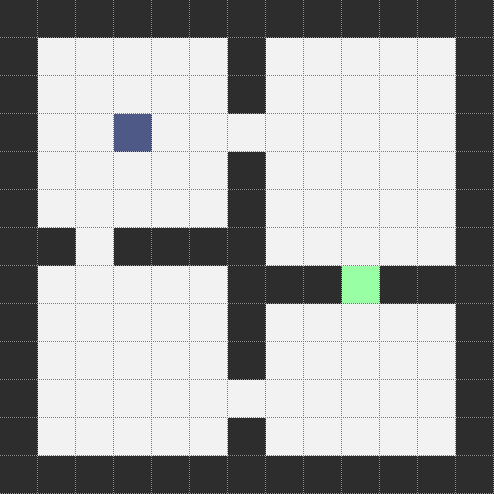
\includegraphics[width=1.2in]{4Rooms.png}
		\caption{The Four Room environment. The black cells indicate the wall. The white cells indicate the area the agents can be in. The blue cell indicates the current position of the agent. The green cell indicates the goal.}
	\end{figure}
	\section{Related Work}
	\qquad \ In this section, some option discovery algorithms will be summarized.
	\subsection*{Option-Critic}
	\qquad \ Option-Critic \cite{bacon2016optioncritic} is an RL algorithm inspired by Action-Critic \cite{Konda00actor-criticalgorithms}, where options are trained to maximize expected return, while an option-value function $Q_\Omega$ is trained to evaluate the decision the options.
	\subsection*{Deliberation Cost}
	\qquad \ Since optimal policy can be achieved even without using options, if options are trained only to maximize expected return, they may degenerate and either terminate every steps or never terminate. Deliberation Cost \cite{harb2017waiting} is a way to encourage longer option duration by punishing option switching.
	\subsection*{Interest Option-Critic}
	\qquad \ The original Option-Critic assumes that options can be initiated everywhere, Interest Option-Critic \cite{khetarpal2020options} tries to remove this assumption by introducing interest functions $I:\mathcal{S} \times \Omega \rightarrow [0,1]$ as a replacement for the initiation set. Experimental result shows that options learned by Interest Option-Critic is localized.
	\subsection*{Termination-Critic}
	\qquad \ Termination-Critic \cite{harutyunyan2019termination} changes the objective of the termination function $\beta$ from maximizing the expected return to minimize the entropy of the termination state. Since entropy can be interpreted as the information gain, this means minimizing the information gained from knowing the termination state, or in other words, making the termination state more predictable.
	\subsection*{Attention Option-Critic}
	\qquad \ Attention Option-Critic \cite{attentionoptioncritic} implements attention mechanism into Option-Critic. Different options are trained to attend to different features of the state. The attention units were trained to not only maximize the expected return, but also other things like maximizing difference between attention of different options.
	\section{Exploration}
	\qquad \ An analysis on localization will be conducted in this section.
	\subsection*{What is Localization?}
	\qquad \ Localization is about options each responsible for a sub-task, or another way of looking at it is options each representing a skill. However, defining and measuring localization quantitatively is hard, which is why most work evaluate these option discovery algorithms qualitatively, by observing the agent acting for an episode in the environment. For example in the Four Rooms environment, only using one option in each room is considered as localization.
	\begin{figure}[h]
		\centering
		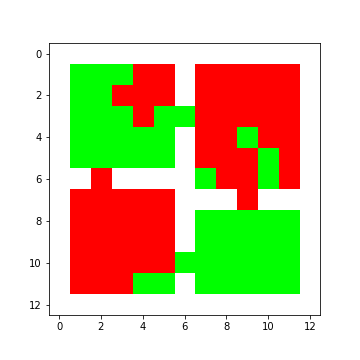
\includegraphics[width=1.6in]{cherryPicked.png}
		\caption{Red and green each represents an option, the options are pretty localized here.}
	\end{figure}
	\subsection*{Why Localization?}
	\qquad \ To understand why we want localization, first we need to answer a fundamental question: Why do we even use options in the first place? Is it to maximize expected return? However, optimal policy can be achieved using only primitive actions. If options cannot give us a higher return, why do we even need options? Some researchers suggest that options should speed up planning \cite{harb2017waiting} \cite{harutyunyan2019termination} and also options should be transferable \cite{khetarpal2020options} \cite{attentionoptioncritic}.
	
	\quad If this is what a good option should be like, then a set of localized options would be beneficial. Localized options are easy to interpret, which made it easily reusable when transferred to a different environment. Also, easy-to-interpret options can speed up planning because each options have its clear purpose and usage.
	\subsection*{How Localization is achieved?}
	\qquad \ Now I will analyze how some of the previous work achieve localization of options.\vspace{0.15in}\\
	\large{\bfseries{Attention Option-Critic}}\vspace{0.05in}
	
	\normalsize{\quad In Attention Option-Critic \cite{attentionoptioncritic}, each options are trained to attend to different features of the state. My hypothesis is that the attention mechanism can act as a constraint on what kind of policy each option can have. Each features of the state represents a piece of information about the state. When performing a sub-task, not all the features are necessary. Each sub-task requires different subset of features. Since the attention mechanism limits the subset of features given to an option, the option cannot learn sub-task that requires features outside of the subset of features it was given, or else the option will perform poorly. In the algorithm, each option is trained to have diverse attention, which force each option to learn to complete a different sub-task.
		
	\quad For example, there is 3 options and an RGB 2D image is the features of the state. Suppose the 3 options each attend to one of the RGB channels, and one of the sub-tasks is checking if there is a purple circle on the image. In this case, only the option with attention on the green channel can complete this sub-task.}
	\begin{figure}[h]
		\centering
		\large{(a)}
		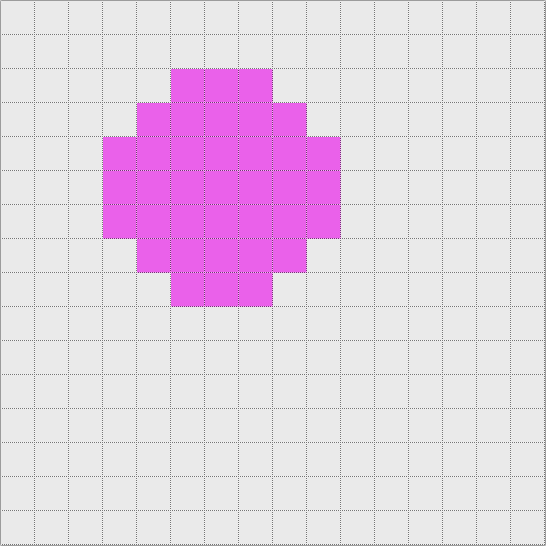
\includegraphics[width=1.2in]{rgb.png}\\
		\large{(b)}
		
\includegraphics[width=1.2in]{rb.png}
		\hspace{0.2in}
		\large{(c)}
		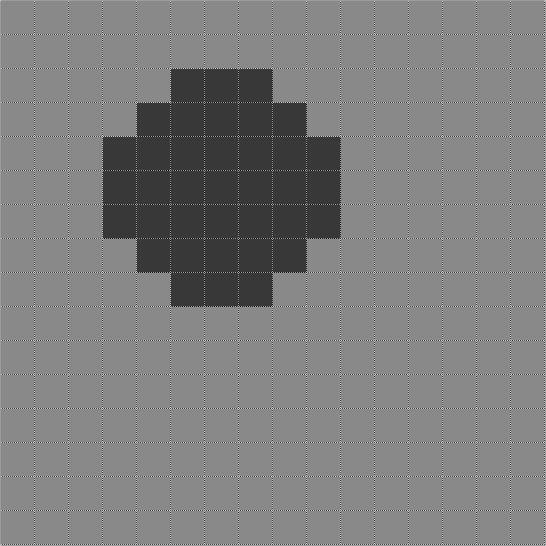
\includegraphics[width=1.2in]{g.png}
		\hspace{0.2in}
		\large{(d)}
		
\includegraphics[width=1.2in]{rb.png}
		\caption{(a) is the RGB input, (b), (c) and (d) are the red, green and blue channel respectively. The circle can only be seen in the green channel.}
	\end{figure}\vspace{0.15in}\\
	\large{\bfseries{Deliberation Cost}}\vspace{0.05in}
	
	\normalsize{\quad In Deliberation Cost \cite{harb2017waiting}, options are encouraged to be more temporally extended. Since options that terminates every step must be non-localized, Deliberation Cost can increase the chance of achieving localization.}\vspace{0.15in}\\
	\large{\bfseries{Termination-Critic}}\vspace{0.05in}
	
	\normalsize{\quad In Termination-Critic \cite{harutyunyan2019termination}, option termination states' entropy is being minimized, and experimental results show that option trained by this usually choose to terminate in bottleneck states (frequently visited states). My hypothesis is that bottleneck states are usually the start or end of a sub-task, having the option terminate at these states essentially chains termination with initiation.
		
	\quad I will illustrate this with a simple example: In the Four Rooms environment, assume that the sub-task is walking from one doorway to another. The two doorway are bottleneck states because the agent must go through them. Since the agent can take on many paths, all the other states are not bottleneck states. When the agent get to the next doorway, another option can be immediately initiated.}
	\begin{figure}[h]
		\centering
		\large{(a)}
		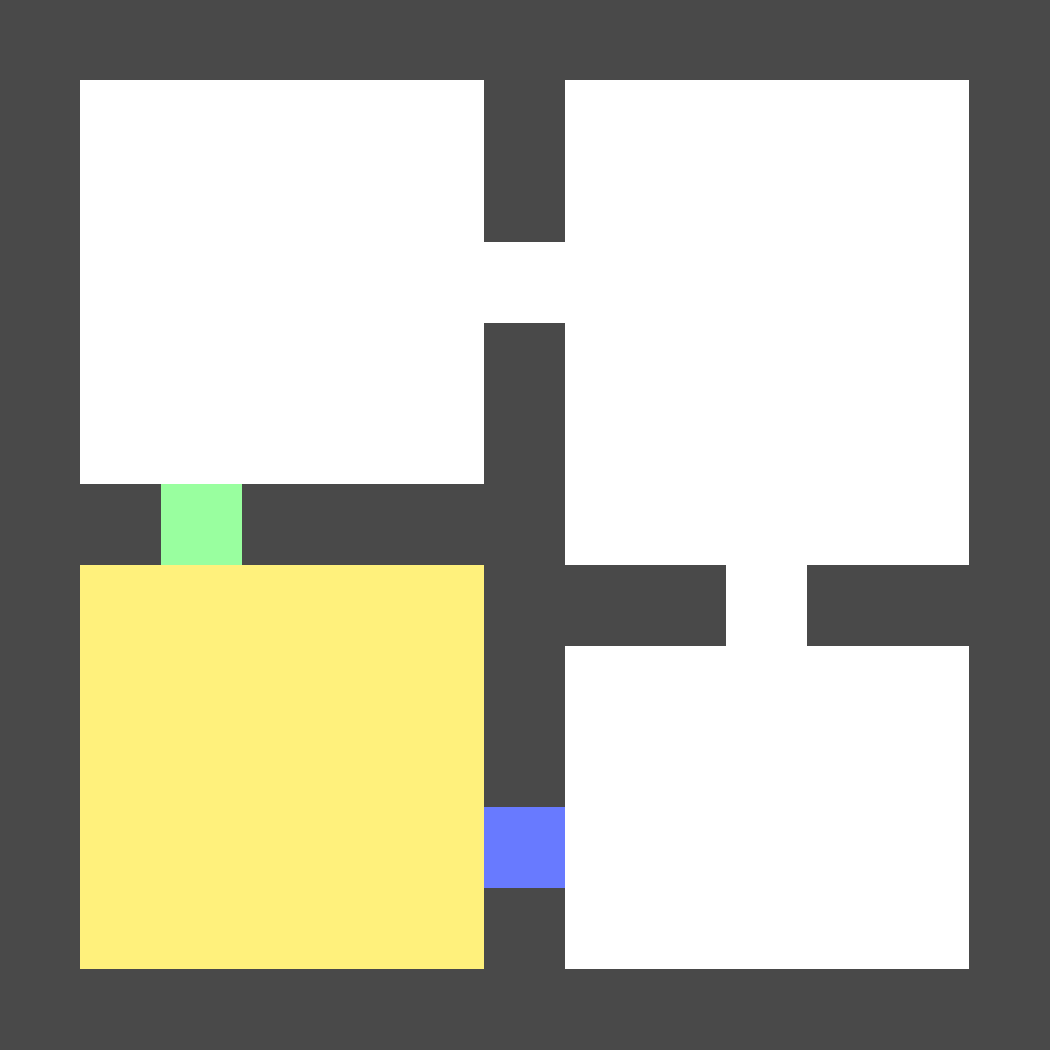
\includegraphics[width=1.2in]{termCrit1.png}
		\hspace{0.2in}
		\large{(b)}
		
\includegraphics[width=1.2in]{termCrit2.png}
		\hspace{0.2in}
		\large{(c)}
		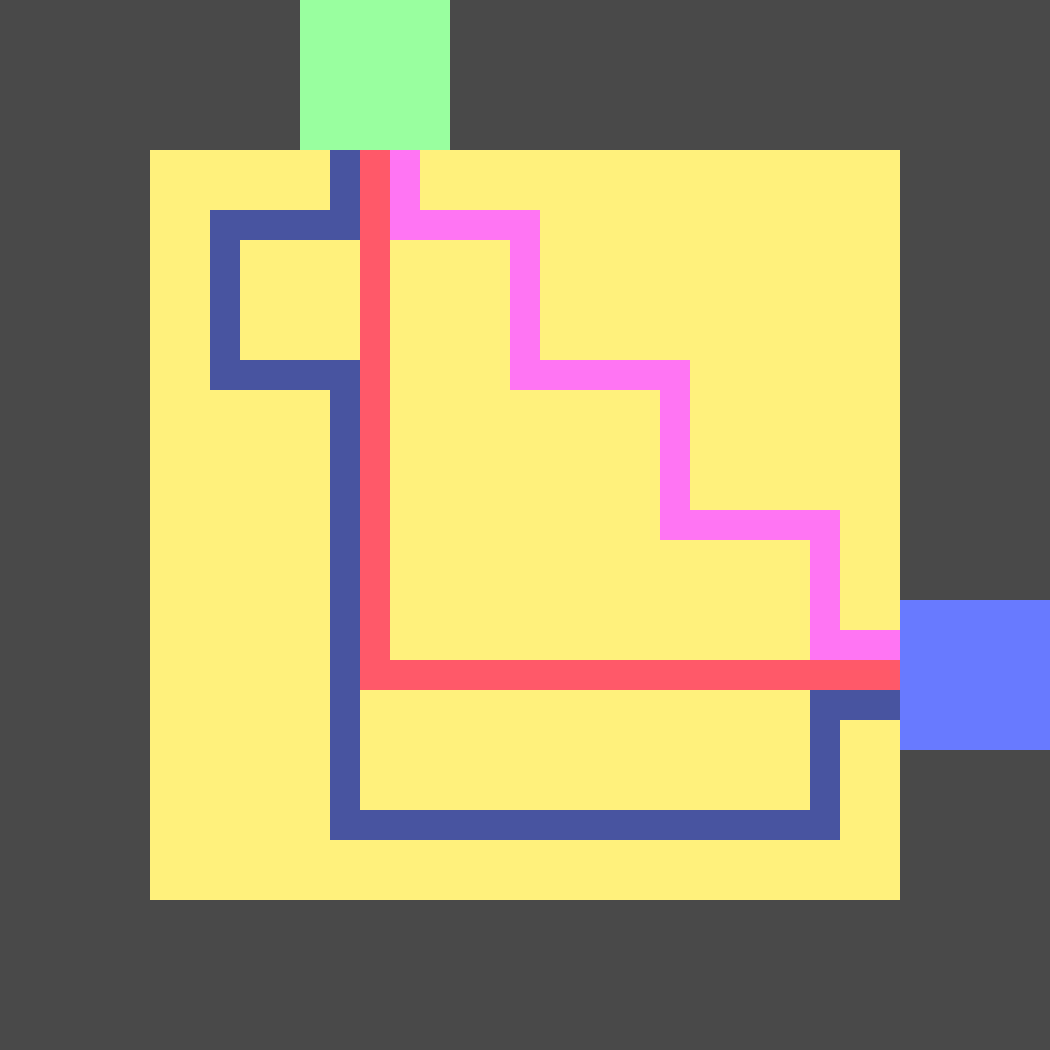
\includegraphics[width=1.2in]{termCrit3.png}
		\caption{(a) and (b) are two options in the theoretic example. Green is the start of the option, blue is the end of the option, yellow is the intermediate states the option may encounter. (c) is a zoomed-in version of the bottom left room. Dark blue, red and pink lines are some of the paths the option can take.}
	\end{figure}\vspace{0.15in}\\
	\large{\bfseries{Interest Option-Critic}}\vspace{0.05in}

	\normalsize{\quad In Interest Option-Critic. My hypothesis is that the interest function made the policy-over-options bias to choosing one of the options in a state, and since the paper uses a neural network as the interest function, the policy-over-options will also bias to choosing that option in a neighboring states.}
	\section{The Localization Framework}
	\qquad \ Naturally, the next question that will be asked is: What do all of these algorithms have in common? Now I will propose a framework that can act as an abstraction for all of these algorithms.\vspace{0.1in}\\
	\rule{420pt}{2pt}\vspace{0.1in}\\
	\large{\bfseries{The Localization Framework}}\\
	\rule{420pt}{0.4pt}\\
	\normalsize{\bfseries{1. Grouping}}
	
	\normalsize{Group states into meaningful sub-tasks based on a certain criterion}\\
	{\bfseries{2. Assignment}}
	
	\normalsize{Assign the sub-tasks to different options}\\
	{\bfseries{3. Optimization}}
	
	\normalsize{Train options to perform well in the sub-task it is given and also improve the initial grouping of sub-tasks}\\
	{\bfseries{4. Selection}}
	
	\normalsize{Form the policy-over-options to select option in different state}\\
	\rule{420pt}{2pt}\vspace{0.1in}
	
	\quad This framework is inspired by Adaboost \cite{adaboost}, which is an Ensemble Learning algorithm from Supervised Learning. There are a lot of similarities between Ensemble Learning and Option Learning, this has already been pointed out in previous work \cite{zhang2018ace}, the individual weak classifiers can be thought of as options.
	
	\quad Each weak classifier is responsible for classifying a small subset of the training data, just like how each option is responsible for a sub-task. In Adaboost, a bunch of weak classifiers are trained sequentially, each of them focuses on training data that is classified poorly by the previous weak classifiers.
	
	\quad Since this training process involves dividing training example into groups, then assign it to different weak classifiers, it inspires the Grouping and Assignment steps in the Localization Framework. Also, the Optimization step in the framework is reminiscent of the weak classifiers learning to classify the training examples. After a lot of weak classifiers are trained, Adaboost combines them together to form a boosted classifier. The boosted classifier is the weighted sum of all the weak classifiers, the weighting is somewhat like a selection process, so it inspires the Selection step in the framework.
	\begin{table}[H]
		\begin{center}
			\begin{tabular}{|p{23mm}||p{30mm}|p{30mm}|p{30mm}|p{30mm}|}
				\hline
				&&&&\\
				&\centering \bfseries Grouping&\centering \bfseries Assignment&\centering \bfseries Optimization&\bfseries \hspace{0.25in} Selection \\
				\hline\hline
				&&&&\\
				\bfseries Attention Option-Critic&\small Group states that need the same sets of features&\small The algorithm assign an attention mechanism to each option&\small Options and attention mechanisms maximize return &\small Choose the option with maximum expected return\\
				&&&&\\
				\hline
				&&&&\\
				\bfseries Termination-Critic&\small Group states between two bottleneck states&\small Each option terminates in a bottleneck state&\small Internal policy maximize return, termination function minimize entropy&\small Choose the option with maximum expected return\\
				&&&&\\
				\hline
				&&&&\\
				\bfseries Interest Option-Critic&\small Group states that are close together&\small The algorithm assign an interest function to each option&\small Options and interest functions maximize return &\small Choose the option with high expected return and interest\\
				&&&&\\
				\hline
			\end{tabular}
			\caption{Previously mentioned algorithms can be fitted into the Localization Framework}
		\end{center}
	\end{table}
	This framework is the abstraction of algorithms that produce localized options, so it is very useful in deriving a new algorithm in the next section.
	\section{Attention-Over-Actions Option-Critic}
	\qquad \ Now that there is a framework, I can just follow the framework and derive a new algorithm. The following algorithm will be called Attention-Over-Actions Option-Critic because it perform abstraction on the action space, this algorithm is largely inspired by Attention Option-Critic.
	\begin{figure}[h]
		\centering
		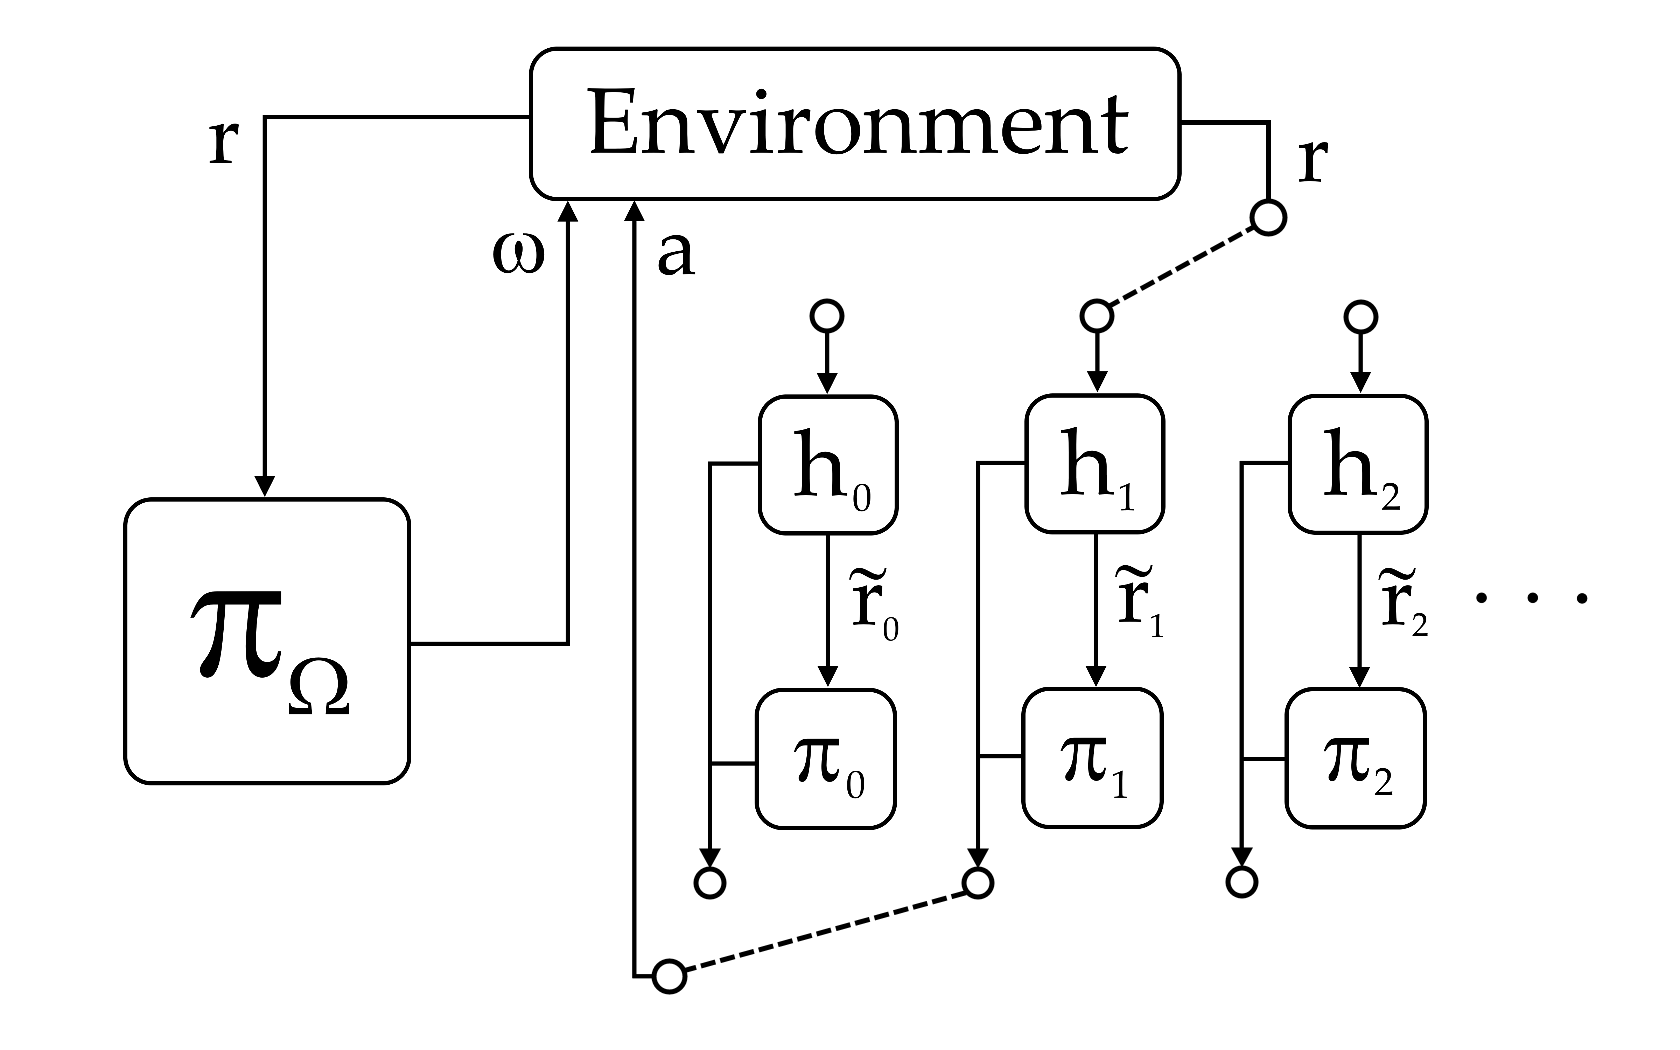
\includegraphics[width=3.8in]{aoaoc.png}
		\caption{Visualization of the interaction between the environment and the Attention-Over-Actions Option-Critic algorithm.}
	\end{figure}
	\subsection*{1. Grouping}
	\qquad \ In Attention Option-Critic, the Grouping step identify sub-tasks based on features needed, this works because each sub-task requires a different subset of features. The following algorithm borrow the idea of attention over state features and apply it to actions, so each option will attend to a different sets of actions. 
	
	\quad The intuition for this is that each sub-task will not need to use all the actions, for example, you would not consider performing a kicking action when you are driving a car. This is essentially performing actions abstraction, since the option can only attend to a subset of the actions.
	\subsection*{2. Assignment}
	\qquad \ The following algorithm assigns the sub-task in a similar way as Attention Option-Critic, an attention mechanism $h_{\omega,\phi}:\mathcal{A} \rightarrow [0,1]$ parameterized by $\phi$ will be given to each option. But instead of masking the state features, it masks the probability for choosing each actions. So the final probability $\pi_{h_\omega}$ for option $\omega$ to choose action $a$ will be: $$\pi_{h_\omega}(a|s) = \frac{\pi_{\omega,\theta}(a|s)h_{\omega, \phi}(a)}{\sum_{a'} \pi_{\omega,\theta}(a'|s)h_{\omega, \phi}(a')}$$ \qquad \ where $\pi_{\omega,\theta}$ is the internal policy of option $\omega$ and is parameterized by $\theta$.
	\subsection*{3. Optimization}
	\qquad \ The optimization of the attention mechanism and that of the option will be described separately.\vspace{0.2in}\\
	{\bfseries Option Optimization}\vspace{0.05in}
	
	\quad Let's first consider the optimization of the option. I will train the internal policy and termination function just like in Option-Critic. They will maximize the expected return by using gradient ascent:
	$$\theta \leftarrow \theta + \alpha_\theta \nabla_\theta Q_\Omega(s,\omega)$$
	$$\nu \leftarrow \nu + \alpha_\nu \nabla_\nu U_\Omega(s',\omega)$$
	\qquad \ where $\theta$ and $\nu$ are the parameters for the internal policy and termination function respectively, $Q_\Omega(s,\omega)$ and $U_\Omega(s',\omega)$ are the expected return for choosing the option $\omega$ in state $s$ and entering the state $s$ when using option $\omega$ respectively.
	
	\quad I can directly reuse the result from the Option-Critic paper:
	$$\nabla_\theta Q_\Omega(s,\omega) = E[\nabla_\theta \log \pi_{\omega, \theta}(a|s) Q_U(s,\omega,a)]$$
	$$\nabla_\nu U_\Omega(s',\omega) = E[\nabla_\nu \beta_{\omega, \nu}(s') A(s',\omega)]$$
	\qquad where $Q_U(s,\omega,a)$ is the expected return for choosing action $a$ when using option $\omega$ in state $s$.
	
	\quad The reason why I ignored the attention mechanism here is that the internal policy should not know the about the attention mechanism, or else it may want to revert the effect of the attention mechanism, i.e. Assigning a high weight to an action with low attention.\vspace{0.2in}\\
	{\bfseries Attention Mechanism Optimization}\vspace{0.05in}
	
	\quad Now let's consider the optimization of $h_{\omega,\phi}$. I want the grouping to be different for all options because or else all options will just aim for the sub-task with highest return. I also want the options to focus on as little actions as possible while still having acceptable performance. Essentially what I need is the algorithm to consider the trade-off between these objectives and achieve a balance between them. A nice way to do this is to add all of these objective up and then perform gradient ascent on the sum: $$\phi \leftarrow \phi + \alpha_\phi \nabla_\phi \sum_{o} (w_o O_o)$$ \qquad \ where $o$ is the index of an objective, $w_o$ is the weight of the objective, $O_o$ is the objective function.
	\quad This method has been used for Attention Option-Critic too. Now I will list out the objectives that I want the option to consider: 
	
	\qquad 1. Perform well
	
	\qquad 2. Different from other options
	
	\qquad 3. The components of the attention mechanism is close to 0 or 1
	
	\qquad 4. Focus on small set of actions
	
	\quad For the first objective, I can just use $Q_\Omega(s,\omega)$ like in Attention Critic. $$\max_h O_1=\max_h Q_\Omega(s,\omega)$$
	
	\quad For the second objective, I will minimize cosine similarity just like in Attention Critic.$$\min_h O_2 = \min_h \sum_{h' \neq h} C(h, h') = \min_h \sum_{h' \neq h} \frac{<h', h>}{||h'||\times||h||}$$
	
	\quad For the third objective, I will minimize entropy in the attention mechanism. Entropy measures the uncertainty in a probability distribution, so $h$ should be normalized first. $$\max_h O_3 = \max_h H(\frac{h}{||h||}) =\max_h <\frac{h}{||h||},\log \frac{h}{||h||}>$$
	
	\quad For the forth objective, I will minimize the length of the attention mechanism, which discourage focusing on too many actions. $$\min_h O_4 = \min_h ||h||$$
	
	\subsection*{4. Selection}
	\qquad \ Any policy-over-options that favor higher Q-value options will work in this case, because the option will need the right set of actions in order to perform well, or else it will fail horribly. So the Q-value already encoded which option has the right set of actions. This means that policies like $\epsilon$-greedy should work for this algorithm.
	
	\begin{algorithm}[H]
	\caption{Pseudocode for Attention-Over-Actions Option-Critic (AOAOC)}
	\begin{algorithmic}
		\vspace{1.5mm}
		\State $s \leftarrow s_0$
		\State Choose $\omega$ according to the policy-over-options $\pi_\Omega(s)$
		\Repeat
		\State Choose $a$ according to $\pi_{h_\omega}(a|s)$
		\State Take action $a$ in $s$, observe $s'$, $r$\vspace{3mm}
		\State \bfseries{1. Options evaluation:}
		\State \normalfont $\delta \leftarrow r - Q_U(s,\omega,a)$
		\If{$s'$ is non-terminal}
		\State $\delta \leftarrow \delta+\gamma(1-\beta_{\omega,\nu}(s'))Q_\Omega(s',\omega)+\gamma \beta_{\omega,\nu}(s')\max_{\omega'}Q_\Omega(s',\omega')$
		\EndIf
		\State $Q_U(s,\omega,a)\leftarrow Q_U(s,\omega,a) + \alpha \delta$
		\vspace{3mm}
		\State {\bfseries1. Options improvement:}
		\State $\theta \leftarrow \theta + \alpha_\theta \nabla_\theta \log \pi_{\omega, \theta}(a|s)Q_U(s,\omega,a)$
		\State $\nu \leftarrow \nu + \alpha_\nu \nabla_\nu \beta_{\omega,\nu}(s')(Q_\Omega(s',\omega)-V_\Omega(s'))$
		\State \normalfont $\phi \leftarrow \phi + \alpha_\phi \nabla_\phi \sum_{o} (w_o O_o)$
		\If{$\beta_{\omega,\nu}$ terminates in $s'$}
		\State {choose new $\omega$ according to the policy-over-options $\pi_\Omega(s)$}
		\EndIf
		\State $s \leftarrow s'$
		\Until $s'$ is terminal	
	\end{algorithmic}
	\end{algorithm}
	\section{Experiment}
	\qquad \ In this section the algorithm AOAOC will be tested in the Four Rooms environment.
	\subsection*{Initial Setup of the Experiment}
	\qquad \ $Q_\Omega$ and $Q_U$ each is represented as a tensor. I do not need to use a neural network here since the state space is discrete in Four Rooms.
	
	\quad $\pi_\Omega$ is an $\epsilon$-greedy policy for the $Q_\Omega$, i.e. the policy-over-options has a probability of $1-\epsilon+\frac{\epsilon}{n_\Omega}$ to select the best option, where $n_\Omega$ is the number of options.
	
	\quad $\nu$ is a tensor, and $\beta_{\omega, \nu}$ is parameterized by $\nu$. More precisely, $\beta_{\omega, \nu} = \sigma(\nu)$, where $\sigma$ is the sigmoid function $\frac{1}{1+e^{-x}}$. This can ensure that $\beta_{\omega, \nu}$ is a probability.
	
	\quad $\theta$ is also a tensor, and $\pi_{\omega, \theta}$ is parameterized by $\theta$. More precisely, $\pi_{\omega, \theta}$ is the softmax over the components of different actions in $\theta$. This can ensure that $\pi_{\omega, \theta}$ is a probability distribution over actions.
	
	\quad $\phi$ is also a tensor, and $h_{\omega, \phi}$ is parameterized by $\phi$. Just like as $\beta_{\omega, \nu}$, $h_{\omega, \phi} = \sigma(\phi)$. This can ensure that $h_{\omega, \phi}$ is between 0 and 1.

	\quad Also, I would like the agent to have a larger incentive to go to the goal in a shorter duration, so I added a punishment of -2 for each step taken by the agent.
	\subsection*{Problematic Attention Mechanism}
	\qquad \ When running the experiment, two problem is encountered:
	
	\qquad 1. The attention mechanism $h_\omega$ often becomes all one. 
	
	\qquad 2. The attention objectives conflict with one another.
	
	\quad Problem 1 leads to degenerate attention mechanism because the option is paying the same amount of attention to all actions. Suppose each of the component in the attention mechanism is a constant $k$, i.e. $h_\omega = [k, k, k, ...]$. The final policy will be:
	$$\pi_{h_\omega}(a|s) = \frac{k \times \pi_\omega(a|s)}{\sum_{a'} k \times \pi_\omega(a'|s)} = \frac{\pi_\omega(a|s)}{\sum_{a'}\pi_\omega(a'|s)}$$
	which is the same as not using attention at all.
	
	\quad This problem is probably caused by the objective 1, which is to maximizing $Q_\Omega(s,\omega)$. Having a uniform attention always yield a higher return because there will not be a constraint to which action it can use.
	\begin{figure}[h]
		\centering
		\small{(a)}
		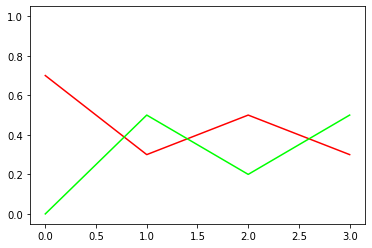
\includegraphics[width=2in]{attentionViz.png}
		\hspace{0.2in}
		\small{(b)}
		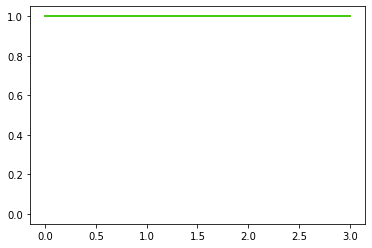
\includegraphics[width=2in]{all1s.png}
		\hspace{0.2in}
		\caption{x-axis is the actions. y-axis is the attention on that action. Red and green lines each represents an attention mechanism. (a) is what the attention mechanism should look like. (b) is when it becomes all ones.}
	\end{figure}

	\quad Problem 2 is follows directly from problem 1. Objective 1 will try to increase all the components to 1. Objective 3 will try to make only one of the components to 1, while the others all 0. Objective 4 will try to decrease all the components to 0.
	
	\quad My original intention is that the algorithm will automatically balance each objective and find the optimal attention mechanism. However, it turns out that the attention mechanism almost always result in 1 of 3 situations:
	
	\qquad 1. All components are 1
	
	\qquad 2. All components are 0
	
	\qquad 3. Only 1 of the component is one, while the others are all zero
	
	\quad For most of the time, 1 of the objectives completely dominates and results in 1 of the 3 situations above. In order to resolve this problem, I can try controlling the number of actions that an option can attend to. However, this will lead to the attention being designed by me instead of being learned by the algorithm, since I have too much control over the training process. Moreover, the desire number of actions for each options are not clear anyway. 
	\begin{figure}[h]
		\centering
		\small{(a)}
		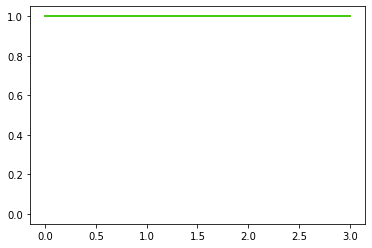
\includegraphics[width=1.5in]{all1s.png}
		\hspace{0.2in}
		\small{(b)}
		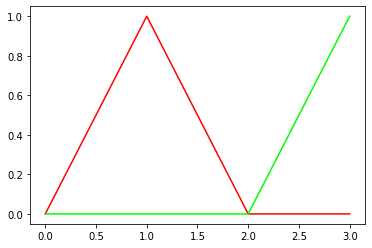
\includegraphics[width=1.5in]{entropyMin.png}
		\hspace{0.2in}
		\small{(c)}
		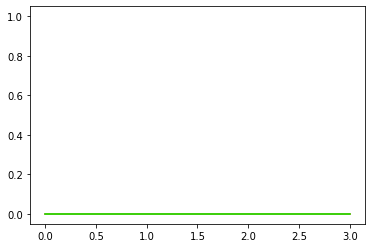
\includegraphics[width=1.5in]{all0s.png}
		\caption{(a), (b) and (c) is the perfect end result for objective 1,3 and 4 respectively. All of which are degenerated attention mechanism.}
	\end{figure}

	\quad In order to solve both of these problems, I decided to limit the attention mechanism to be a probability distribution. Instead of using a sigmoid function, I will use a softmax function for the attention mechanism.
	
	\quad This has a lot of benefit, for instance, the objective 4 can be eliminated because a probability distribution need to add up to 1 anyway. Also, the situation where all the components of the attention mechanism becomes 0 or 1 will not happened. This change also makes intuitive sense, since as you pay more attention to one thing, you pay less attention to others.
	\subsection*{Adding Deliberation Cost}
	\qquad \ One way of qualitatively evaluating the algorithm's ability to create localized options is to look at the $Q_\Omega$ in each state. If the options are localized, the state space will be clearly divided into regions. However, this is not the case.
	\begin{figure}[h]
		\centering
		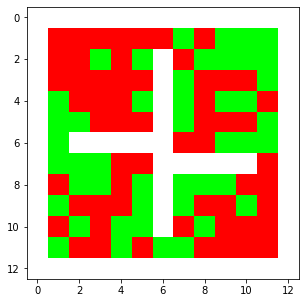
\includegraphics[width=1.5in]{noDC.png}
		\caption{The option that will be chosen in each state. Red and green cell each corresponds to 1 of the options. In this figure, the options are not localized.}
	\end{figure}

	\quad This is not completely unreasonable, because the algorithm has no reason to group actions that are being used successively together. So I decided to add deliberation cost to the algorithm. I will now provide a simple scenario to illustrate why I added deliberation cost.
	\begin{figure}[h]
	\centering
	\small{(a)}
	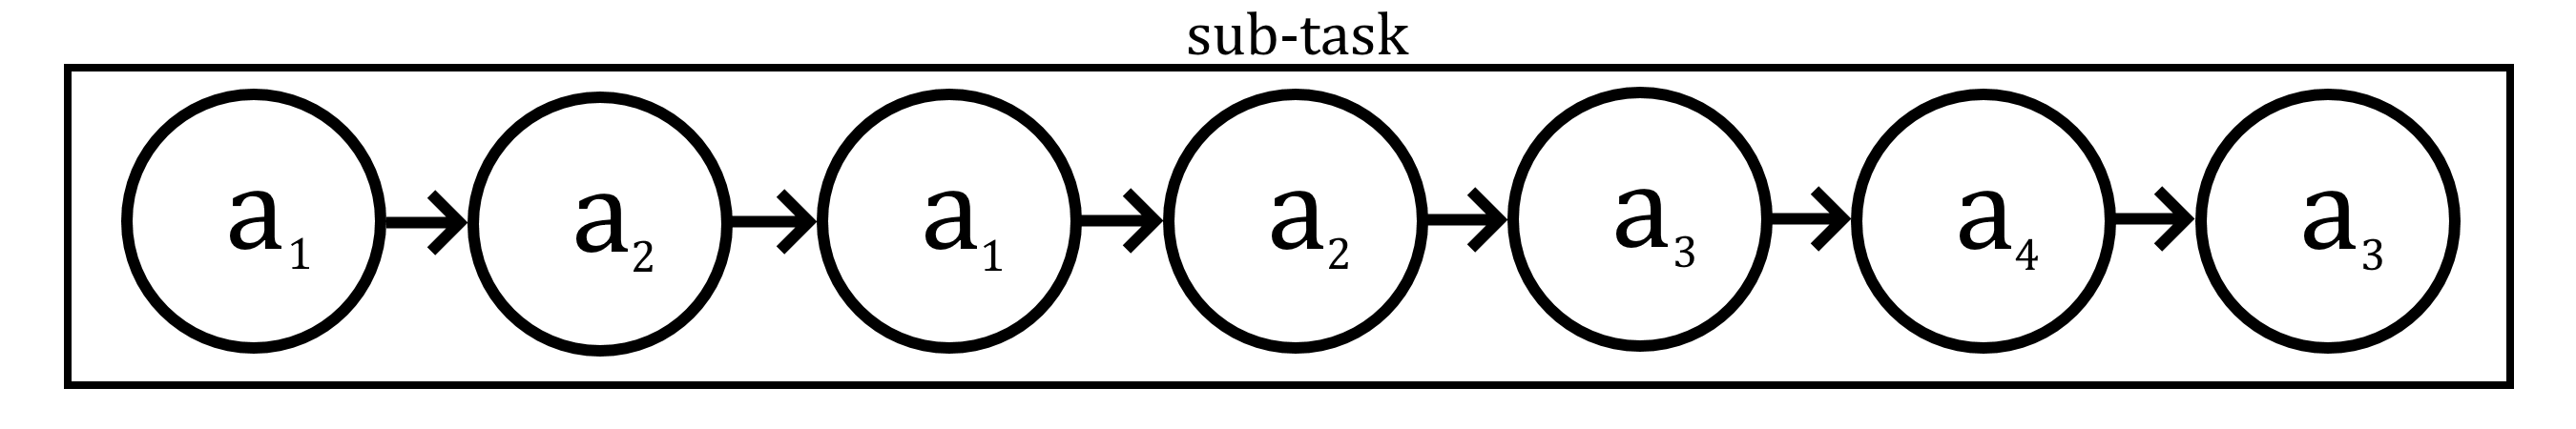
\includegraphics[width=4in]{actionSeq.png}\\
	\small{(b)}
	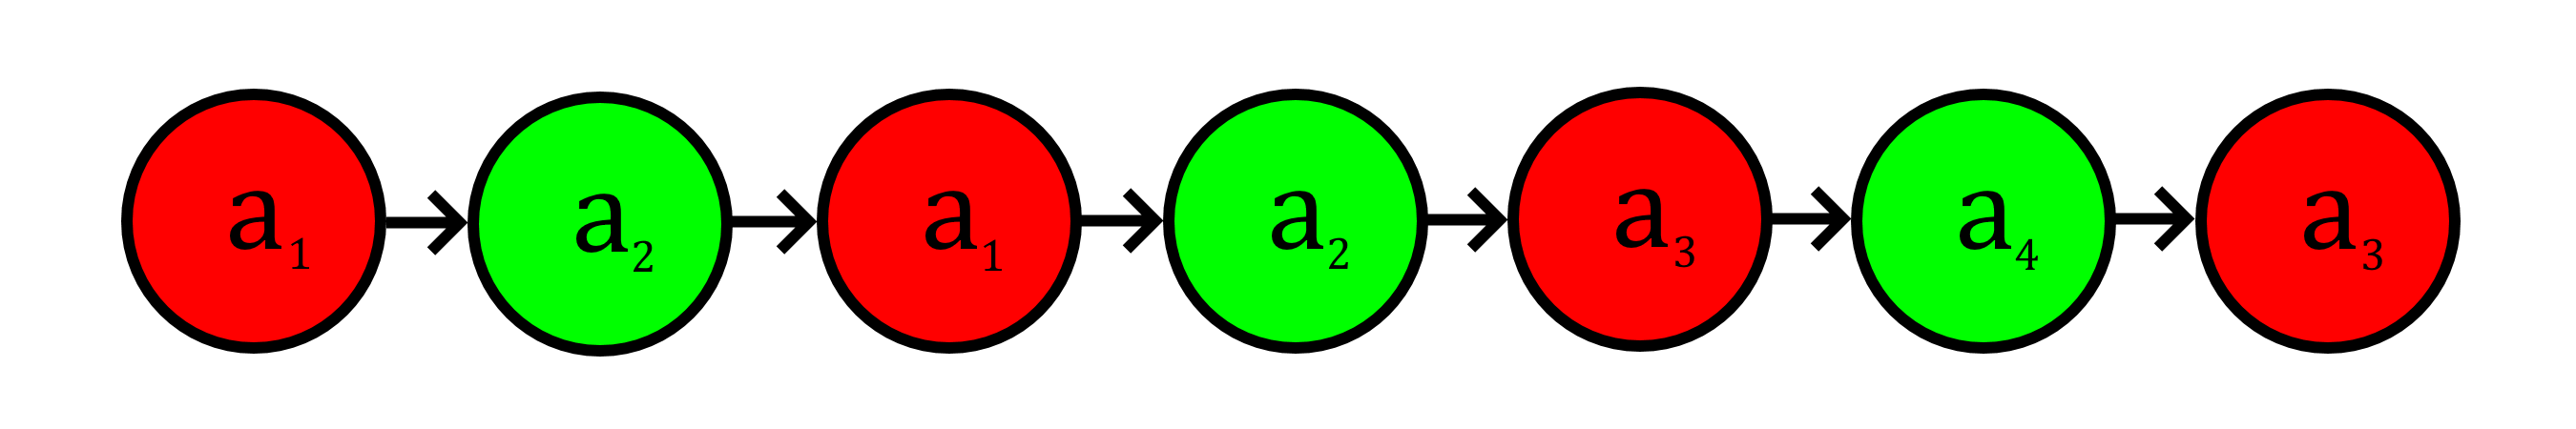
\includegraphics[width=4in]{actionSeqB.png}\\
	\small{(c)}
	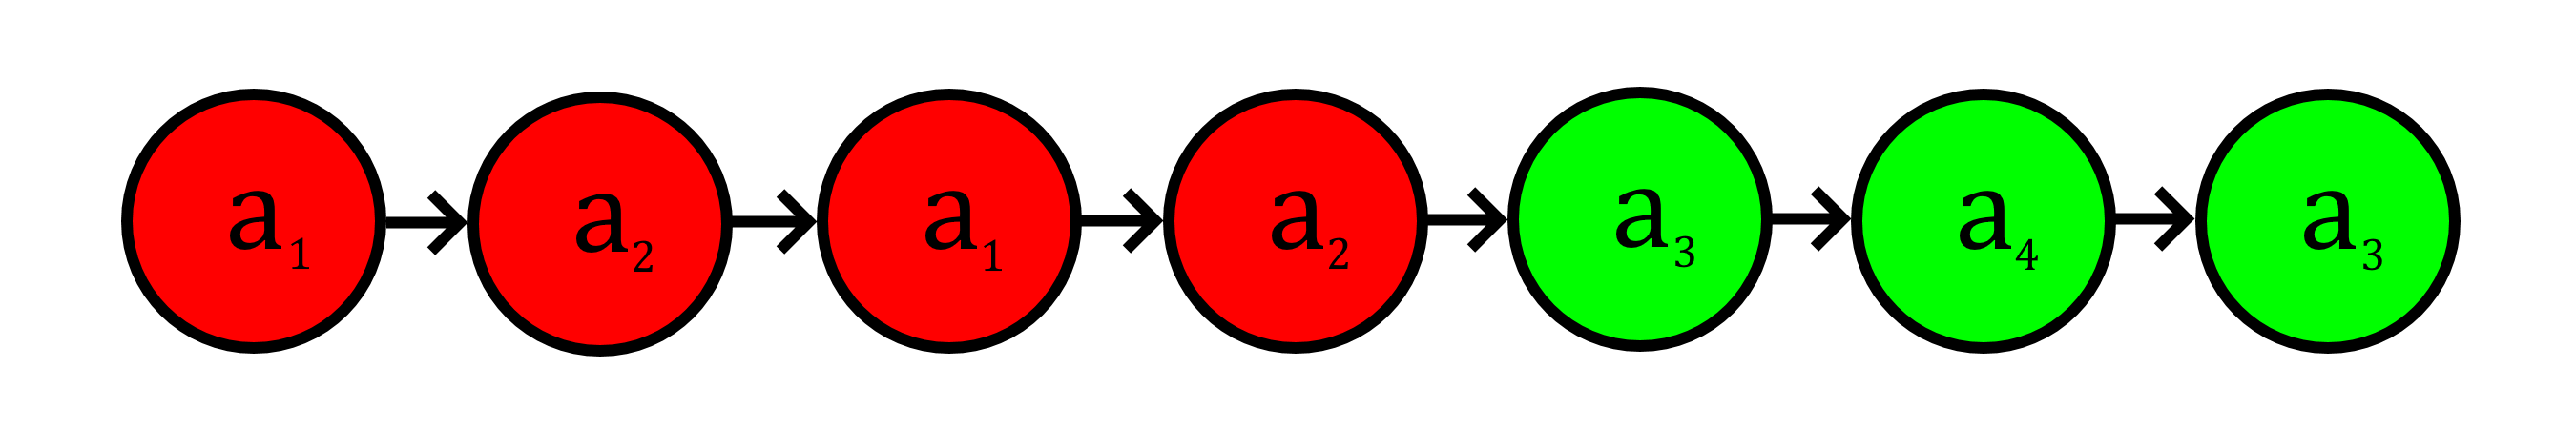
\includegraphics[width=4in]{actionSeqG.png}
	\caption{(a) is the hypothetical sub-task. Red and green each corresponds to 1 of the options. (b) and (c) corresponds to not using and using deliberation cost respectively. In (b), the red option attends to $a_1,a_3$, the green option attends to $a_2,a_4$. In (c), the red option attends to $a_1,a_2$, the green option attends to $a_3,a_4$.}
	\end{figure}
	
	\quad Suppose $a_1, a_2, a_3, a_4$ are actions, and there is a sub-task where first you have to perform $a_1$ and $a_2$ in an alternating fashion, then after a while, you have to perform $a_3$ and $a_4$ also in an alternating fashion.
	
	\quad Without deliberation cost, the algorithm has no reason not to make one option attend to $a_1$ and $a_3$, another option attend to $a_2$ and $a_4$. However, with deliberation cost, the algorithm will make one option attend to $a_1$ and $a_2$, another option attend to $a_3$ and $a_4$, because this will decrease the deliberation cost.

	\quad Note that the deliberation cost used here uses $\tau = 0$.
	
	\quad Adding deliberation cost can also be interpreted as adding an extra constraint to the original deliberation cost algorithm, so that apart from having long options, options should also use a small set of actions.
	\subsection*{Comparison with Deliberation Cost}
	\qquad \ Indeed it is able to divide the state space into regions. However, when comparing this with the original deliberation cost algorithm, it is not clear what benefit has the attention mechanism brought. 
	\begin{figure}[h]
		\centering
		\large{(a)}
		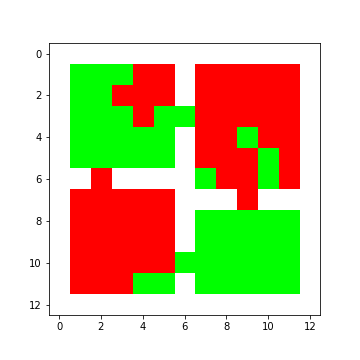
\includegraphics[width=1.5in]{cherryPicked.png}
		\hspace{0.2in}
		\large{(b)}
		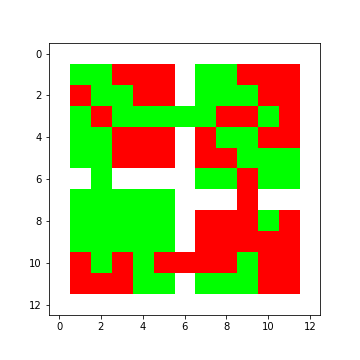
\includegraphics[width=1.5in]{nonPicked.png}
		\caption{Localization only occurs sometimes. (a) is a cherry-picked result that localization has been achieved. (b) is what the result looks with the same hyperparameters.}
	\end{figure}

	\quad AOAOC with deliberation cost and Deliberation Cost alone seem to produce pretty similar results. This means that probably the localization is only achieved because of the deliberation cost.
	
	\quad Even though there seems to be no benefit in using attention mechanism from the above results, in theory, localized options produced by AOAOC should be more meaningful than that produced by deliberation cost. Deliberation cost group states that are close together into a sub-task, while AOAOC should group actions that are used consecutively into a sub-task.
	
	\quad This is why I changed the environment to make it easier. I switched the left and right action in the top-right and bottom-left room. This way navigating each room should only need 2 of the actions, and also the 2 actions needed in a room is completely different from its neighboring rooms.
	\begin{figure}[h]
		\centering
		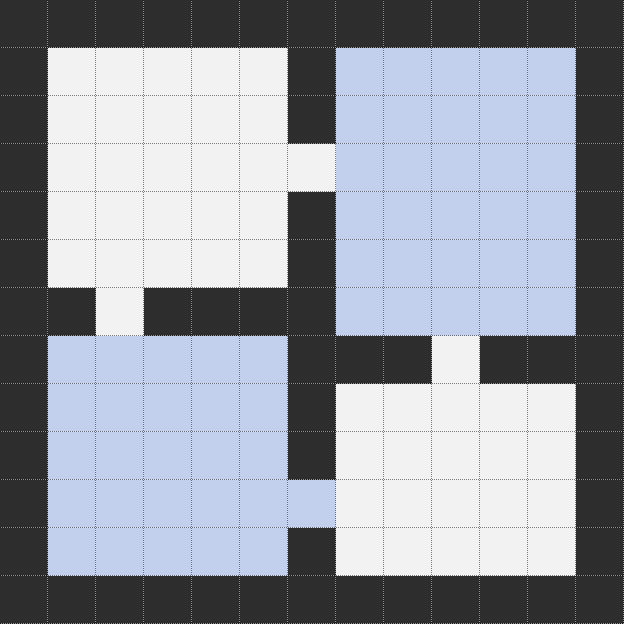
\includegraphics[width=1.5in]{after.png}
		\caption{The left and right actions in the blue area is switched. So in the white area, only the up and right actions are needed. While in the blue area, only the down and left actions are needed.}
	\end{figure}

	\quad sort of success but may be overfitting
	\section{Conclusion}
	\qquad \ 
	\section{Future Direction}
	\qquad \ As mentioned before, this algorithm probably can only work in environment with large discrete action space. Hence, a possible future direction is trying to apply this in an environment which has a large action space.
	
	\quad Besides, the idea of this algorithm can also be extended to continuous action space. In continuous action space sometimes the action will be a vector, the options can attend to only some of the components of this action vector.
	\section*{Bibliography}
	\bibliographystyle{ieeetr}
	\bibliography{bibliography}
		
	\section*{Appendix}
	\appendix
	\section{Notations}
	{\bfseries Markov Decision Process}\\
	$\mathcal{S}$ --- Set of states\\
	$\mathcal{A}$ --- Set of actions\\
	$r$ --- Reward function or reward\\
	$\gamma$ --- Discount factor\\
	$P$ --- Transition model\\
	$\pi$ --- Policy\\
	$s$ --- State\\
	$a$ --- Action\\
	$s_T$ --- Terminal state\vspace{0.1in}\\
	{\bfseries Option Framework}\\
	$\Omega$ --- Set of options\\
	$\pi_{\omega,\theta}$ --- Internal policy of option $\omega$\\
	$\beta_\omega$ --- Termination probability of option $\omega$\\
	$\mathcal{I}_\omega$ --- Initiation set of option $\omega$\\
	$\pi_\Omega$ --- Policy-over-options\\
	$Q_U$ --- Expected return for choosing an action\\
	$Q_\Omega$ --- Expected return for choosing an option\\
	$A_\Omega$ --- Expected advantage for choosing an option\\
	$V_\Omega$ --- Expected return in a state\\
	$U_\Omega$ --- Expected return for arriving in a state\\
	$\theta$ --- Parameter for internal policy\\
	$\nu$ --- Parameter for termination probability\\
	$\omega$ --- option\vspace{0.1in}\\
	{\bfseries Attention-Over-Actions Option-Critic}\\
	$h_{\omega,\phi}$ --- Attention Mechanism\\
	$\pi_{h_\omega}$ --- Final probability\\
	$\phi$ --- Parameter for attention mechanism\\
	$\alpha$ --- Learning rate for $Q_U$\\
	$\alpha_\theta$ --- Learning rate for internal policy\\
	$\alpha_\nu$ --- Learning rate for termination probability\\
	$\alpha_\phi$ --- Learning rate for attention mechanism\\
	$O_o$ --- Objective function\\
	$w_o$ --- Weight of objective function\\
	$o$ --- Objective\\
	$\delta$ --- One step Q-value error\vspace{0.1in}\\
	{\bfseries Operations}\\
	$\nabla$ --- Gradient\\
	$E[\ ]$ --- Expected value\\
	$\leftarrow$ --- Assignment\\
	$<,>$ --- Dot product\\
	$||.||$ --- Length of a vector\\
	\section{Proof}
	\subsection{Derivative of Objective 1}
	Let $h_\omega^a$ be the element in the attention vector $h_\omega$ that corresponds to the action $a$, i.e. $h_\omega = [h_\omega^{a_0}, h_\omega^{a_1}, ...]$
	$$\frac{\partial Q_\Omega(s,\omega)}{\partial h_\omega^a} = \sum_{s,\omega} \mu_\Omega(s,\omega|s_0, \omega_0)\sum_a \frac{\partial \pi_{h_\omega} (a|s)}{\partial h_\omega^a} Q_U(s,\omega,a)$$
	$$= E_{s,\omega,a \sim \pi_{h_\omega}}[\frac{\partial \log \pi_{h_\omega}(a|s)}{\partial h_\omega^a}Q_U(s,\omega,a)]$$
	The steps above follows directly from the Option-Critic appendix. The next step is to express $\frac{\partial \log \pi_{h_\omega} (a|s)}{\partial h_\omega^a}$ in a simpler form.
	$$\frac{\partial \log \pi_{h_\omega} (a|s)}{\partial h_\omega^a} = \frac{\partial}{\partial h_\omega^a} [\log\frac{\pi_\omega(a|s)h_\omega^a}{\sum_{a'} \pi_\omega(a'|s)h_\omega^{a'}}]$$
	$$=\frac{\partial}{\partial h_\omega^a} [\log\pi_\omega(a|s) + \log h_\omega^a - \log\sum_{a'}\pi_\omega(a'|s)h_\omega^{a'}]$$
	$$=\frac{\partial}{\partial h_\omega^a} [\log\pi_\omega(a|s)] + \frac{\partial}{\partial h_\omega^a}[\log h_\omega^a] - \frac{\partial}{\partial h_\omega^a}[\log\sum_{a'}\pi_\omega(a'|s)h_\omega^{a'}]$$
	$\pi_\omega(a|s)$ is independent of $h_\omega^a$, hence $\frac{\partial}{\partial h_\omega^a} [\log\pi_\omega(a|s)]=0$
	$$= \frac{\partial}{\partial h_\omega^a}[\log h_\omega^a] - \frac{\partial}{\partial h_\omega^a}[\log\sum_{a'}\pi_\omega(a'|s)h_\omega^{a'}]$$
	$$= \frac{1}{h_\omega^a} - \frac{\pi_\omega(a|s)}{\sum_{a'}\pi_\omega(a'|s)h_\omega^{a'}}$$
	$$= \frac{1}{h_\omega^a} - \frac{\pi_\omega(a|s)}{\sum_{a'}\pi_\omega(a'|s)h_\omega^{a'}} \times \frac{h_\omega^a}{h_\omega^a}$$
	By definition $\pi_{h_\omega}(a|s)=\frac{\pi_\omega(a|s)h_\omega^a}{\sum_{a'} \pi_\omega(a'|s)h_\omega^{a'}}$
	$$= \frac{1}{h_\omega^a} - \frac{\pi_{h_\omega}(a|s)}{h_\omega^a}$$
	$$= \frac{1-\pi_{h_\omega}(a|s)}{h_\omega^a}$$
	Substitute back to the original calculation,
	$$\frac{\partial Q_\Omega(s,\omega)}{\partial h_\omega^a} = E_{s,\omega,a \sim \pi_{h_\omega}}[\frac{1-\pi_{h_\omega}(a|s)}{h_\omega^a}Q_U(s,\omega,a)]$$
	\subsection{Derivative of Objective 2}
	Let $h_\omega^a$ be the element in the attention vector $h_\omega$ that corresponds to the action $a$, i.e. $h_\omega = [h_\omega^{a_0}, h_\omega^{a_1}, ...]$
	Since we would like to minimize the cosine similarity, the negative cosine similarity will be used instead.
	$$\sum_{h_{\omega '} \neq h_\omega} \frac{\partial C(h_\omega, h_{\omega '})}{\partial h_\omega^a} = \sum_{h_{\omega '} \neq h_\omega} \frac{\partial}{\partial h_\omega^a} \frac{<h_\omega, h_{\omega '}>}{||h_\omega||\times||h_{\omega '}||}$$
	$$= \sum_{h_{\omega '} \neq h_\omega} \frac{||h_\omega||\times||h_{\omega '}|| \frac{\partial}{\partial h_\omega^a} <h_\omega, h_{\omega '}> - <h_\omega, h_{\omega '}> \frac{\partial}{\partial h_\omega^a} ||h_\omega||\times||h_{\omega '}||}{(||h_\omega||\times||h_{\omega '}||)^2}$$
	I will calculate each of the derivative separately:
	$$\frac{\partial}{\partial h_\omega^a} <h_\omega, h_{\omega '}> = \frac{\partial}{\partial h_\omega^a} \sum_{a'}h_\omega^{a'} h_{\omega '}^{a'} = h_{\omega '}^a$$
	$$\frac{\partial}{\partial h_\omega^a} ||h_\omega||\times||h_{\omega '}|| = ||h_{\omega '}|| \frac{\partial}{\partial h_\omega^a} \sqrt{\sum_{a'}(h_\omega^{a'})^2} = ||h_{\omega '}|| \frac{h_\omega^a}{\sqrt{\sum_{a'}(h_\omega^{a'})^2}}$$
	Substitute back to the original calculation,
	$$\sum_{h_{\omega '} \neq h_\omega} \frac{\partial}{\partial h_\omega^a} \frac{<h_\omega, h_{\omega '}>}{||h_\omega||\times||h_{\omega '}||} = \sum_{h_{\omega '} \neq h_\omega} \frac{||h_\omega||\times||h_{\omega '}|| h_{\omega '}^a - <h_\omega, h_{\omega '}> ||h_{\omega '}|| \frac{h_\omega^a}{\sqrt{\sum_{a'}(h_\omega^{a'})^2}}}{(||h_\omega||\times||h_{\omega '}||)^2}$$
	$$= \sum_{h_{\omega '} \neq h_\omega} \frac{h_{\omega '}^a}{||h_\omega||\times||h_{\omega '}||} - \frac{<h_\omega, h_{\omega '}> h_\omega^a}{(||h_\omega||\times||h_{\omega '}||)\times||h_{\omega}||^2}$$
	\subsection{Derivative of Objective 3}
	Let $h_\omega^a$ be the element in the attention vector $h_\omega$ that corresponds to the action $a$, i.e. $h_\omega = [h_\omega^{a_0}, h_\omega^{a_1}, ...]$
	Since entropy usually applies to probabilities, I will normalize the attention unit into $\overline{h_\omega} = \frac{h_\omega}{\sum_{a'} h_\omega^{a'}}$
	$$\frac{\partial H(\overline{h_\omega})}{\partial h_\omega^a} = \frac{\partial \sum_{a'} \overline{h_\omega^{a'}}\log \overline{h_\omega^{a'}}}{\partial h_\omega^a}$$
	$$= \frac{\partial \overline{h_\omega^a} \log \overline{h_\omega^a}}{\partial h_\omega^a} + \sum_{\overline{h_\omega^{a'}} \neq \overline{h_\omega^{a}}} \frac{\partial \overline{h_\omega^{a'}} \log \overline{h_\omega^{a'}}}{\partial h_\omega^{a'}}$$
	$$= \frac{\partial \overline{h_\omega^a} \log \overline{h_\omega^a}}{\partial \overline{h_\omega^{a}}} \times \frac{\partial \overline{h_\omega^a}}{h_\omega^a} + \sum_{\overline{h_\omega^{a'}} \neq \overline{h_\omega^{a}}} \frac{\partial \overline{h_\omega^{a'}} \log \overline{h_\omega^{a'}}}{\partial \overline{h_\omega^{a'}}} \times \frac{\partial \overline{h_\omega^{a'}}}{h_\omega^{a'}}$$
	I will calculate each of the derivative separately:
	$$\frac{\partial \overline{h_\omega^a} \log \overline{h_\omega^a}}{\partial \overline{h_\omega^{a}}} = \log \overline{h_\omega^a}\frac{\partial \overline{h_\omega^a}}{\partial \overline{h_\omega^{a}}} + \overline{h_\omega^a}\frac{\partial \log \overline{h_\omega^a}}{\partial \overline{h_\omega^{a}}} = \log \overline{h_\omega^a} + 1$$
	$$\frac{\partial \overline{h_{\omega}^a}}{\partial h_\omega^a} = \frac{\partial}{\partial h_\omega^a} \frac{h_\omega^a}{\sum_b h_\omega^b} = \frac{\sum_b h_\omega^b - h_\omega^a}{(\sum_{b} h_\omega^b)^2}$$
	$$\frac{\partial \overline{h_{\omega}^{a'}}}{\partial h_\omega^a} = \frac{\partial}{\partial h_\omega^a} \frac{h_\omega^{a'}}{\sum_b h_\omega^b} = \frac{- h_\omega^{a'}}{(\sum_b h_\omega^b)^2}$$
	Substitute back to the original calculation,
	$$\frac{\partial \overline{h_\omega^a} \log \overline{h_\omega^a}}{\partial \overline{h_\omega^{a}}} = (\log \overline{h_\omega^a} + 1)\frac{\sum_b h_\omega^b - h_\omega^a}{(\sum_{b} h_\omega^b)^2} + \sum_{\overline{h_\omega^{a'}} \neq \overline{h_\omega^{a}}} (\log \overline{h_\omega^{a'}} + 1)\frac{- h_\omega^{a'}}{(\sum_b h_\omega^b)^2}$$
	$$=\frac{(\log \overline{h_\omega^a} + 1)}{\sum_b h_\omega^b} + \sum_{h_\omega^{a'}} (\log \overline{h_\omega^{a'}} + 1)\frac{- h_\omega^{a'}}{(\sum_b h_\omega^b)^2}$$
	\subsection{Derivative of Objective 4}
	Let $h_\omega^a$ be the element in the attention vector $h_\omega$ that corresponds to the action $a$, i.e. $h_\omega = [h_\omega^{a_0}, h_\omega^{a_1}, ...]$
	Since we would like to minimize the length, the negative length will be used instead.
	$$\frac{\partial ||h_\omega||}{\partial h_\omega^a} = \frac{\partial}{\partial h_\omega^a} \sqrt{\sum_{a'} (h_\omega^{a'})^2}$$
	$$= \frac{h_\omega^a}{\sqrt{\sum_{a'} (h_\omega^{a'})^2}} = \frac{h_\omega^a}{||h_\omega||}$$
	\section{Experimental Details}
	\section{Experimental Results}
	\subsection*{AOAOC in Unmodified Four Rooms}
	\begin{figure}[H]
		\centering
		\begin{tabular}{ccccc}
			\subfloat{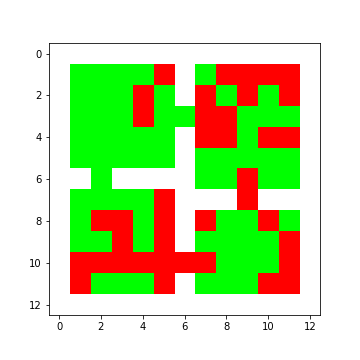
\includegraphics[width=0.85in]{result/aoaoc_hard/wo_0.01/dc_1/run_0.png}} &
			\subfloat{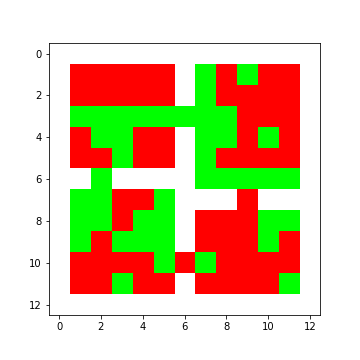
\includegraphics[width=0.85in]{result/aoaoc_hard/wo_0.01/dc_1/run_1.png}} &
			\subfloat{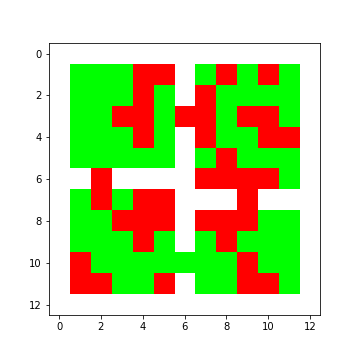
\includegraphics[width=0.85in]{result/aoaoc_hard/wo_0.01/dc_1/run_2.png}} &
			\subfloat{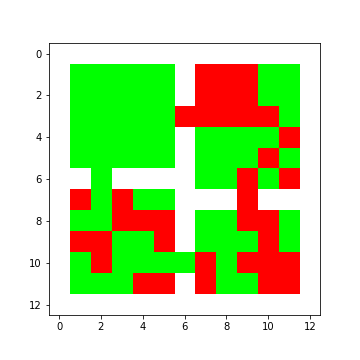
\includegraphics[width=0.85in]{result/aoaoc_hard/wo_0.01/dc_1/run_3.png}} &
			\subfloat{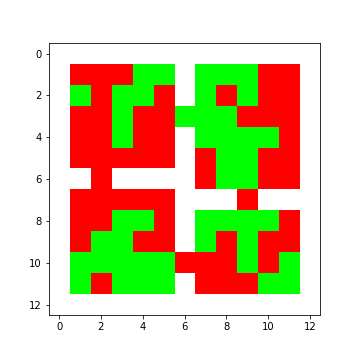
\includegraphics[width=0.85in]{result/aoaoc_hard/wo_0.01/dc_1/run_4.png}} \\		\subfloat{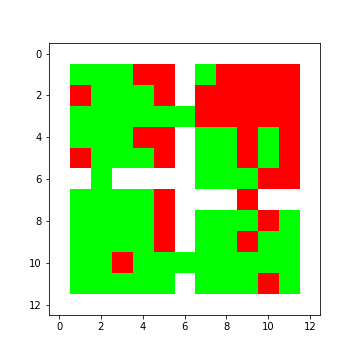
\includegraphics[width=0.85in]{result/aoaoc_hard/wo_0.05/dc_1/run_0.png}} &
			\subfloat{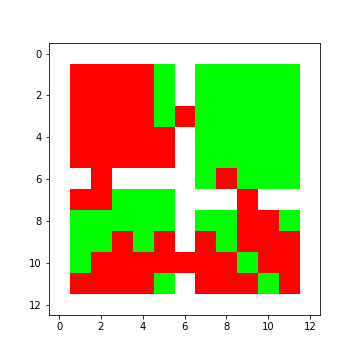
\includegraphics[width=0.85in]{result/aoaoc_hard/wo_0.05/dc_1/run_1.png}} &
			\subfloat{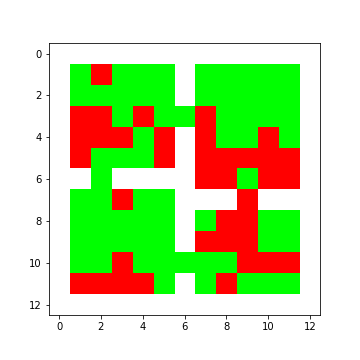
\includegraphics[width=0.85in]{result/aoaoc_hard/wo_0.05/dc_1/run_2.png}} &
			\subfloat{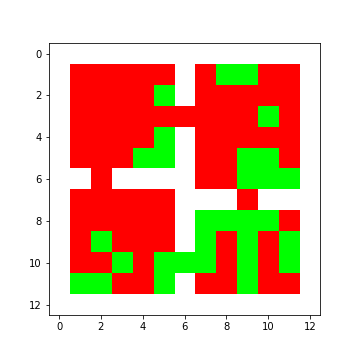
\includegraphics[width=0.85in]{result/aoaoc_hard/wo_0.05/dc_1/run_3.png}} &
			\subfloat{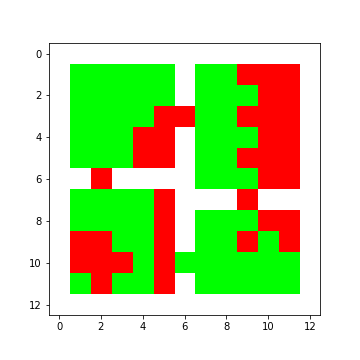
\includegraphics[width=0.85in]{result/aoaoc_hard/wo_0.05/dc_1/run_4.png}} \\
			\subfloat{\includegraphics[width=0.85in]{result/aoaoc_hard/wo_0.1/dc_1/run_0.png}} &
			\subfloat{\includegraphics[width=0.85in]{result/aoaoc_hard/wo_0.1/dc_1/run_1.png}} &
			\subfloat{\includegraphics[width=0.85in]{result/aoaoc_hard/wo_0.1/dc_1/run_2.png}} &
			\subfloat{\includegraphics[width=0.85in]{result/aoaoc_hard/wo_0.1/dc_1/run_3.png}} &
			\subfloat{\includegraphics[width=0.85in]{result/aoaoc_hard/wo_0.1/dc_1/run_4.png}} \\
			\subfloat{\includegraphics[width=0.85in]{result/aoaoc_hard/wo_0.2/dc_1/run_0.png}} &
			\subfloat{\includegraphics[width=0.85in]{result/aoaoc_hard/wo_0.2/dc_1/run_1.png}} &
			\subfloat{\includegraphics[width=0.85in]{result/aoaoc_hard/wo_0.2/dc_1/run_2.png}} &
			\subfloat{\includegraphics[width=0.85in]{result/aoaoc_hard/wo_0.2/dc_1/run_3.png}} &
			\subfloat{\includegraphics[width=0.85in]{result/aoaoc_hard/wo_0.2/dc_1/run_4.png}} \\
		\end{tabular}
		\caption{Deliberation Cost = 1. Learning rate of attention mechanism = 0.01, 0.05, 0.1 and 0.2 from top to bottom. Same row means same hyperparameters, each column is a different trial. }
	\end{figure}
	\begin{figure}[H]
	\centering
	\begin{tabular}{ccccc}
		\subfloat{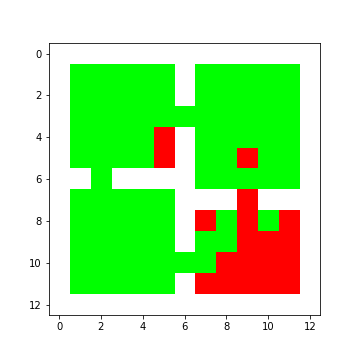
\includegraphics[width=0.85in]{result/aoaoc_hard/wo_0.01/dc_2/run_0.png}} &
		\subfloat{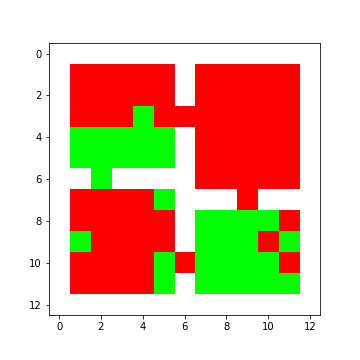
\includegraphics[width=0.85in]{result/aoaoc_hard/wo_0.01/dc_2/run_1.png}} &
		\subfloat{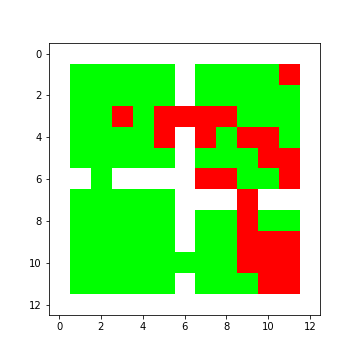
\includegraphics[width=0.85in]{result/aoaoc_hard/wo_0.01/dc_2/run_2.png}} &
		\subfloat{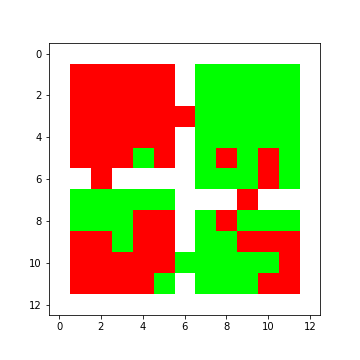
\includegraphics[width=0.85in]{result/aoaoc_hard/wo_0.01/dc_2/run_3.png}} &
		\subfloat{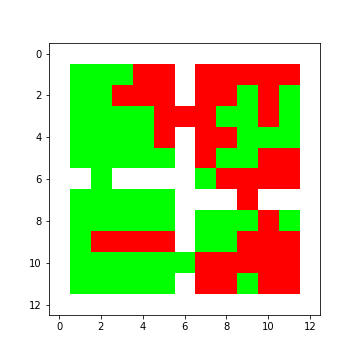
\includegraphics[width=0.85in]{result/aoaoc_hard/wo_0.01/dc_2/run_4.png}} \\
		\subfloat{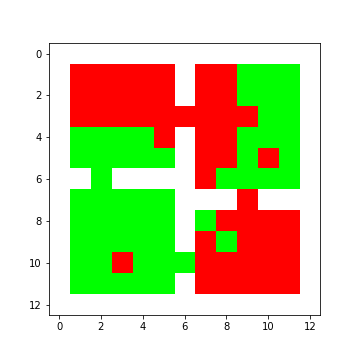
\includegraphics[width=0.85in]{result/aoaoc_hard/wo_0.05/dc_2/run_0.png}} &
		\subfloat{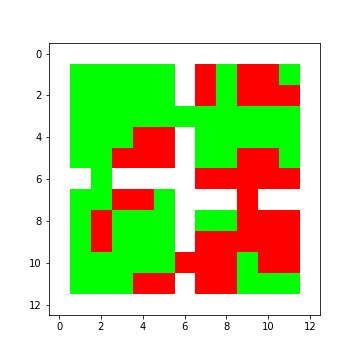
\includegraphics[width=0.85in]{result/aoaoc_hard/wo_0.05/dc_2/run_1.png}} &
		\subfloat{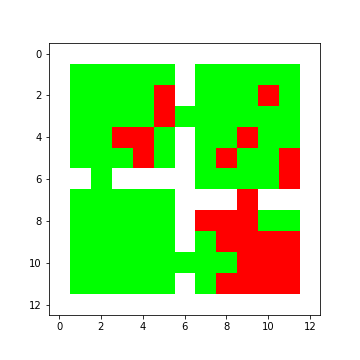
\includegraphics[width=0.85in]{result/aoaoc_hard/wo_0.05/dc_2/run_2.png}} &
		\subfloat{\includegraphics[width=0.85in]{result/aoaoc_hard/wo_0.05/dc_2/run_3.png}} &
		\subfloat{\includegraphics[width=0.85in]{result/aoaoc_hard/wo_0.05/dc_2/run_4.png}} \\
		\subfloat{\includegraphics[width=0.85in]{result/aoaoc_hard/wo_0.1/dc_2/run_0.png}} &
		\subfloat{\includegraphics[width=0.85in]{result/aoaoc_hard/wo_0.1/dc_2/run_1.png}} &
		\subfloat{\includegraphics[width=0.85in]{result/aoaoc_hard/wo_0.1/dc_2/run_2.png}} &
		\subfloat{\includegraphics[width=0.85in]{result/aoaoc_hard/wo_0.1/dc_2/run_3.png}} &
		\subfloat{\includegraphics[width=0.85in]{result/aoaoc_hard/wo_0.1/dc_2/run_4.png}} \\
		\subfloat{\includegraphics[width=0.85in]{result/aoaoc_hard/wo_0.2/dc_2/run_0.png}} &
		\subfloat{\includegraphics[width=0.85in]{result/aoaoc_hard/wo_0.2/dc_2/run_1.png}} &
		\subfloat{\includegraphics[width=0.85in]{result/aoaoc_hard/wo_0.2/dc_2/run_2.png}} &
		\subfloat{\includegraphics[width=0.85in]{result/aoaoc_hard/wo_0.2/dc_2/run_3.png}} &
		\subfloat{\includegraphics[width=0.85in]{result/aoaoc_hard/wo_0.2/dc_2/run_4.png}} \\
	\end{tabular}
	\caption{Deliberation Cost = 2. Learning rate of attention mechanism = 0.01, 0.05, 0.1 and 0.2 from top to bottom. Same row means same hyperparameters, each column is a different trial. }
	\end{figure}
	\begin{figure}[H]
	\centering
	\begin{tabular}{ccccc}
		\subfloat{\includegraphics[width=0.85in]{result/aoaoc_hard/wo_0.01/dc_3/run_0.png}} &
		\subfloat{\includegraphics[width=0.85in]{result/aoaoc_hard/wo_0.01/dc_3/run_1.png}} &
		\subfloat{\includegraphics[width=0.85in]{result/aoaoc_hard/wo_0.01/dc_3/run_2.png}} &
		\subfloat{\includegraphics[width=0.85in]{result/aoaoc_hard/wo_0.01/dc_3/run_3.png}} &
		\subfloat{\includegraphics[width=0.85in]{result/aoaoc_hard/wo_0.01/dc_3/run_4.png}} \\
		\subfloat{\includegraphics[width=0.85in]{result/aoaoc_hard/wo_0.05/dc_3/run_0.png}} &
		\subfloat{\includegraphics[width=0.85in]{result/aoaoc_hard/wo_0.05/dc_3/run_1.png}} &
		\subfloat{\includegraphics[width=0.85in]{result/aoaoc_hard/wo_0.05/dc_3/run_2.png}} &
		\subfloat{\includegraphics[width=0.85in]{result/aoaoc_hard/wo_0.05/dc_3/run_3.png}} &
		\subfloat{\includegraphics[width=0.85in]{result/aoaoc_hard/wo_0.05/dc_3/run_4.png}} \\
		\subfloat{\includegraphics[width=0.85in]{result/aoaoc_hard/wo_0.1/dc_3/run_0.png}} &
		\subfloat{\includegraphics[width=0.85in]{result/aoaoc_hard/wo_0.1/dc_3/run_1.png}} &
		\subfloat{\includegraphics[width=0.85in]{result/aoaoc_hard/wo_0.1/dc_3/run_2.png}} &
		\subfloat{\includegraphics[width=0.85in]{result/aoaoc_hard/wo_0.1/dc_3/run_3.png}} &
		\subfloat{\includegraphics[width=0.85in]{result/aoaoc_hard/wo_0.1/dc_3/run_4.png}} \\
		\subfloat{\includegraphics[width=0.85in]{result/aoaoc_hard/wo_0.2/dc_3/run_0.png}} &
		\subfloat{\includegraphics[width=0.85in]{result/aoaoc_hard/wo_0.2/dc_3/run_1.png}} &
		\subfloat{\includegraphics[width=0.85in]{result/aoaoc_hard/wo_0.2/dc_3/run_2.png}} &
		\subfloat{\includegraphics[width=0.85in]{result/aoaoc_hard/wo_0.2/dc_3/run_3.png}} &
		\subfloat{\includegraphics[width=0.85in]{result/aoaoc_hard/wo_0.2/dc_3/run_4.png}} \\
	\end{tabular}
	\caption{Deliberation Cost = 3. Learning rate of attention mechanism = 0.01, 0.05, 0.1 and 0.2 from top to bottom. Same row means same hyperparameters, each column is a different trial. }
	\end{figure}
	\subsection*{AOAOC in Modified Four Rooms}
	\begin{figure}[H]
	\centering
	\begin{tabular}{ccccc}
		\subfloat{\includegraphics[width=0.85in]{result/aoaoc_easy/wo_0.01/dc_1/run_0.png}} &
		\subfloat{\includegraphics[width=0.85in]{result/aoaoc_easy/wo_0.01/dc_1/run_1.png}} &
		\subfloat{\includegraphics[width=0.85in]{result/aoaoc_easy/wo_0.01/dc_1/run_2.png}} &
		\subfloat{\includegraphics[width=0.85in]{result/aoaoc_easy/wo_0.01/dc_1/run_3.png}} &
		\subfloat{\includegraphics[width=0.85in]{result/aoaoc_easy/wo_0.01/dc_1/run_4.png}} \\
		\subfloat{\includegraphics[width=0.85in]{result/aoaoc_easy/wo_0.05/dc_1/run_0.png}} &
		\subfloat{\includegraphics[width=0.85in]{result/aoaoc_easy/wo_0.05/dc_1/run_1.png}} &
		\subfloat{\includegraphics[width=0.85in]{result/aoaoc_easy/wo_0.05/dc_1/run_2.png}} &
		\subfloat{\includegraphics[width=0.85in]{result/aoaoc_easy/wo_0.05/dc_1/run_3.png}} &
		\subfloat{\includegraphics[width=0.85in]{result/aoaoc_easy/wo_0.05/dc_1/run_4.png}} \\
		\subfloat{\includegraphics[width=0.85in]{result/aoaoc_easy/wo_0.1/dc_1/run_0.png}} &
		\subfloat{\includegraphics[width=0.85in]{result/aoaoc_easy/wo_0.1/dc_1/run_1.png}} &
		\subfloat{\includegraphics[width=0.85in]{result/aoaoc_easy/wo_0.1/dc_1/run_2.png}} &
		\subfloat{\includegraphics[width=0.85in]{result/aoaoc_easy/wo_0.1/dc_1/run_3.png}} &
		\subfloat{\includegraphics[width=0.85in]{result/aoaoc_easy/wo_0.1/dc_1/run_4.png}} \\
		\subfloat{\includegraphics[width=0.85in]{result/aoaoc_easy/wo_0.2/dc_1/run_0.png}} &
		\subfloat{\includegraphics[width=0.85in]{result/aoaoc_easy/wo_0.2/dc_1/run_1.png}} &
		\subfloat{\includegraphics[width=0.85in]{result/aoaoc_easy/wo_0.2/dc_1/run_2.png}} &
		\subfloat{\includegraphics[width=0.85in]{result/aoaoc_easy/wo_0.2/dc_1/run_3.png}} &
		\subfloat{\includegraphics[width=0.85in]{result/aoaoc_easy/wo_0.2/dc_1/run_4.png}} \\
	\end{tabular}
	\caption{Deliberation Cost = 1. Learning rate of attention mechanism = 0.01, 0.05, 0.1 and 0.2 from top to bottom. Same row means same hyperparameters, each column is a different trial. }
	\end{figure}
	\begin{figure}[H]
	\centering
	\begin{tabular}{ccccc}
		\subfloat{\includegraphics[width=0.85in]{result/aoaoc_easy/wo_0.01/dc_2/run_0.png}} &
		\subfloat{\includegraphics[width=0.85in]{result/aoaoc_easy/wo_0.01/dc_2/run_1.png}} &
		\subfloat{\includegraphics[width=0.85in]{result/aoaoc_easy/wo_0.01/dc_2/run_2.png}} &
		\subfloat{\includegraphics[width=0.85in]{result/aoaoc_easy/wo_0.01/dc_2/run_3.png}} &
		\subfloat{\includegraphics[width=0.85in]{result/aoaoc_easy/wo_0.01/dc_2/run_4.png}} \\
		\subfloat{\includegraphics[width=0.85in]{result/aoaoc_easy/wo_0.05/dc_2/run_0.png}} &
		\subfloat{\includegraphics[width=0.85in]{result/aoaoc_easy/wo_0.05/dc_2/run_1.png}} &
		\subfloat{\includegraphics[width=0.85in]{result/aoaoc_easy/wo_0.05/dc_2/run_2.png}} &
		\subfloat{\includegraphics[width=0.85in]{result/aoaoc_easy/wo_0.05/dc_2/run_3.png}} &
		\subfloat{\includegraphics[width=0.85in]{result/aoaoc_easy/wo_0.05/dc_2/run_4.png}} \\
		\subfloat{\includegraphics[width=0.85in]{result/aoaoc_easy/wo_0.1/dc_2/run_0.png}} &
		\subfloat{\includegraphics[width=0.85in]{result/aoaoc_easy/wo_0.1/dc_2/run_1.png}} &
		\subfloat{\includegraphics[width=0.85in]{result/aoaoc_easy/wo_0.1/dc_2/run_2.png}} &
		\subfloat{\includegraphics[width=0.85in]{result/aoaoc_easy/wo_0.1/dc_2/run_3.png}} &
		\subfloat{\includegraphics[width=0.85in]{result/aoaoc_easy/wo_0.1/dc_2/run_4.png}} \\
		\subfloat{\includegraphics[width=0.85in]{result/aoaoc_easy/wo_0.2/dc_2/run_0.png}} &
		\subfloat{\includegraphics[width=0.85in]{result/aoaoc_easy/wo_0.2/dc_2/run_1.png}} &
		\subfloat{\includegraphics[width=0.85in]{result/aoaoc_easy/wo_0.2/dc_2/run_2.png}} &
		\subfloat{\includegraphics[width=0.85in]{result/aoaoc_easy/wo_0.2/dc_2/run_3.png}} &
		\subfloat{\includegraphics[width=0.85in]{result/aoaoc_easy/wo_0.2/dc_2/run_4.png}} \\
	\end{tabular}
	\caption{Deliberation Cost = 2. Learning rate of attention mechanism = 0.01, 0.05, 0.1 and 0.2 from top to bottom. Same row means same hyperparameters, each column is a different trial. }
	\end{figure}
	\begin{figure}[H]
	\centering
	\begin{tabular}{ccccc}
		\subfloat{\includegraphics[width=0.85in]{result/aoaoc_easy/wo_0.01/dc_3/run_0.png}} &
		\subfloat{\includegraphics[width=0.85in]{result/aoaoc_easy/wo_0.01/dc_3/run_1.png}} &
		\subfloat{\includegraphics[width=0.85in]{result/aoaoc_easy/wo_0.01/dc_3/run_2.png}} &
		\subfloat{\includegraphics[width=0.85in]{result/aoaoc_easy/wo_0.01/dc_3/run_3.png}} &
		\subfloat{\includegraphics[width=0.85in]{result/aoaoc_easy/wo_0.01/dc_3/run_4.png}} \\
		\subfloat{\includegraphics[width=0.85in]{result/aoaoc_easy/wo_0.05/dc_3/run_0.png}} &
		\subfloat{\includegraphics[width=0.85in]{result/aoaoc_easy/wo_0.05/dc_3/run_1.png}} &
		\subfloat{\includegraphics[width=0.85in]{result/aoaoc_easy/wo_0.05/dc_3/run_2.png}} &
		\subfloat{\includegraphics[width=0.85in]{result/aoaoc_easy/wo_0.05/dc_3/run_3.png}} &
		\subfloat{\includegraphics[width=0.85in]{result/aoaoc_easy/wo_0.05/dc_3/run_4.png}} \\
		\subfloat{\includegraphics[width=0.85in]{result/aoaoc_easy/wo_0.1/dc_3/run_0.png}} &
		\subfloat{\includegraphics[width=0.85in]{result/aoaoc_easy/wo_0.1/dc_3/run_1.png}} &
		\subfloat{\includegraphics[width=0.85in]{result/aoaoc_easy/wo_0.1/dc_3/run_2.png}} &
		\subfloat{\includegraphics[width=0.85in]{result/aoaoc_easy/wo_0.1/dc_3/run_3.png}} &
		\subfloat{\includegraphics[width=0.85in]{result/aoaoc_easy/wo_0.1/dc_3/run_4.png}} \\
		\subfloat{\includegraphics[width=0.85in]{result/aoaoc_easy/wo_0.2/dc_3/run_0.png}} &
		\subfloat{\includegraphics[width=0.85in]{result/aoaoc_easy/wo_0.2/dc_3/run_1.png}} &
		\subfloat{\includegraphics[width=0.85in]{result/aoaoc_easy/wo_0.2/dc_3/run_2.png}} &
		\subfloat{\includegraphics[width=0.85in]{result/aoaoc_easy/wo_0.2/dc_3/run_3.png}} &
		\subfloat{\includegraphics[width=0.85in]{result/aoaoc_easy/wo_0.2/dc_3/run_4.png}} \\
	\end{tabular}
	\caption{Deliberation Cost = 3. Learning rate of attention mechanism = 0.01, 0.05, 0.1 and 0.2 from top to bottom. Same row means same hyperparameters, each column is a different trial. }
	\end{figure}
	\subsection*{Deliberation Cost in Unmodified Four Rooms}
	\begin{figure}[H]
		\centering
		\begin{tabular}{ccccc}
			\subfloat{\includegraphics[width=0.85in]{result/dc_hard/dc_0.5/run_0.png}} &
			\subfloat{\includegraphics[width=0.85in]{result/dc_hard/dc_0.5/run_1.png}} &
			\subfloat{\includegraphics[width=0.85in]{result/dc_hard/dc_0.5/run_2.png}} &
			\subfloat{\includegraphics[width=0.85in]{result/dc_hard/dc_0.5/run_3.png}} &
			\subfloat{\includegraphics[width=0.85in]{result/dc_hard/dc_0.5/run_4.png}} \\
			\subfloat{\includegraphics[width=0.85in]{result/dc_hard/dc_1/run_0.png}} &
			\subfloat{\includegraphics[width=0.85in]{result/dc_hard/dc_1/run_1.png}} &
			\subfloat{\includegraphics[width=0.85in]{result/dc_hard/dc_1/run_2.png}} &
			\subfloat{\includegraphics[width=0.85in]{result/dc_hard/dc_1/run_3.png}} &
			\subfloat{\includegraphics[width=0.85in]{result/dc_hard/dc_1/run_4.png}} \\
			\subfloat{\includegraphics[width=0.85in]{result/dc_hard/dc_2/run_0.png}} &
			\subfloat{\includegraphics[width=0.85in]{result/dc_hard/dc_2/run_1.png}} &
			\subfloat{\includegraphics[width=0.85in]{result/dc_hard/dc_2/run_2.png}} &
			\subfloat{\includegraphics[width=0.85in]{result/dc_hard/dc_2/run_3.png}} &
			\subfloat{\includegraphics[width=0.85in]{result/dc_hard/dc_2/run_4.png}} \\
			\subfloat{\includegraphics[width=0.85in]{result/dc_hard/dc_3/run_0.png}} &
			\subfloat{\includegraphics[width=0.85in]{result/dc_hard/dc_3/run_1.png}} &
			\subfloat{\includegraphics[width=0.85in]{result/dc_hard/dc_3/run_2.png}} &
			\subfloat{\includegraphics[width=0.85in]{result/dc_hard/dc_3/run_3.png}} &
			\subfloat{\includegraphics[width=0.85in]{result/dc_hard/dc_3/run_4.png}} \\
		\end{tabular}
		\caption{Deliberation Cost = 0.5, 1, 2 and 3 from top to bottom. Same row means same hyperparameters, each column is a different trial. }
	\end{figure}
	\subsection*{Deliberation Cost in Modified Four Rooms}
	\begin{figure}[H]
	\centering
	\begin{tabular}{ccccc}
		\subfloat{\includegraphics[width=0.85in]{result/dc_easy/dc_0.5/run_0.png}} &
		\subfloat{\includegraphics[width=0.85in]{result/dc_easy/dc_0.5/run_1.png}} &
		\subfloat{\includegraphics[width=0.85in]{result/dc_easy/dc_0.5/run_2.png}} &
		\subfloat{\includegraphics[width=0.85in]{result/dc_easy/dc_0.5/run_3.png}} &
		\subfloat{\includegraphics[width=0.85in]{result/dc_easy/dc_0.5/run_4.png}} \\
		\subfloat{\includegraphics[width=0.85in]{result/dc_easy/dc_1/run_0.png}} &
		\subfloat{\includegraphics[width=0.85in]{result/dc_easy/dc_1/run_1.png}} &
		\subfloat{\includegraphics[width=0.85in]{result/dc_easy/dc_1/run_2.png}} &
		\subfloat{\includegraphics[width=0.85in]{result/dc_easy/dc_1/run_3.png}} &
		\subfloat{\includegraphics[width=0.85in]{result/dc_easy/dc_1/run_4.png}} \\
		\subfloat{\includegraphics[width=0.85in]{result/dc_easy/dc_2/run_0.png}} &
		\subfloat{\includegraphics[width=0.85in]{result/dc_easy/dc_2/run_1.png}} &
		\subfloat{\includegraphics[width=0.85in]{result/dc_easy/dc_2/run_2.png}} &
		\subfloat{\includegraphics[width=0.85in]{result/dc_easy/dc_2/run_3.png}} &
		\subfloat{\includegraphics[width=0.85in]{result/dc_easy/dc_2/run_4.png}} \\
		\subfloat{\includegraphics[width=0.85in]{result/dc_easy/dc_3/run_0.png}} &
		\subfloat{\includegraphics[width=0.85in]{result/dc_easy/dc_3/run_1.png}} &
		\subfloat{\includegraphics[width=0.85in]{result/dc_easy/dc_3/run_2.png}} &
		\subfloat{\includegraphics[width=0.85in]{result/dc_easy/dc_3/run_3.png}} &
		\subfloat{\includegraphics[width=0.85in]{result/dc_easy/dc_3/run_4.png}} \\
	\end{tabular}
	\caption{Deliberation Cost = 0.5, 1, 2 and 3 from top to bottom. Same row means same hyperparameters, each column is a different trial. }
	\end{figure}
	\section{Code}
	The code below is based on codes in the ioc repository.\cite{iocrepo}
	\lstset{style=code}
	\subsection*{fourrooms.py}
	\lstinputlisting[language=Python]{../code/fourrooms.py}
	\subsection*{aoaoc\_tabular.py}
	\lstinputlisting[language=Python]{../code/aoaoc_tabular.py}
	\subsection*{visualize.py}
	\lstinputlisting[language=Python]{../code/visualize.py}
\end{document}